% !TEX root = ../thesis.tex
\graphicspath{{./vega-lang/figures/}}
\chapter{Declarative Primitives for Interaction Design}
\label{sec:vg:lang}

Reactive Vega builds on a long-running thread of research on declarative
visualization design, popularized by the Grammar of
Graphics~\cite{wilkinson:grammar} and Polaris~\cite{stolte:polaris} (now
Tableau).

Visual encodings are defined by composing graphical primitives called
\emph{marks}~\cite{bostock:protovis}, which include \emph{arcs}, \emph{areas},
\emph{bars}, \emph{lines}, plotting \emph{symbols} and \emph{text}. Marks are
associated with datasets, and their specifications map tuple values to visual
properties such as position and color. Scales and guides (i.e., axes and
legends) are provided as first-class primitives for mapping a domain of data
values to a range of visual properties. Special \emph{group} marks serve as
containers to express nested or small multiple displays. Child marks and scales
can inherit a group's data, or draw from independent datasets.

Although interaction is a crucial component of effective
visualization~\cite{liu:mentalmodels, pike:interactionscience}, existing
declarative visualization models, including widely used tools such as
D3~\cite{bostock:d3} and ggplot2~\cite{wickham:ggplot2}, do not offer composable
primitives for interaction design. Instead, if they support interaction, they do
so through either a palette of standard techniques~\cite{bostock:protovis,
bostock:d3} or \emph{imperative} event handling callbacks. While the former
restricts expressivity, the later undoes many of the benefits of declarative
design. In particular, users are forced to contend with interaction execution
details, such as interleaved events and coordinating external state, which can
be complex and error\--prone~\cite{cooper:embedding, edwards:coherent,
myers:callbacks}.

\begin{figure}[h!]
  \centering
  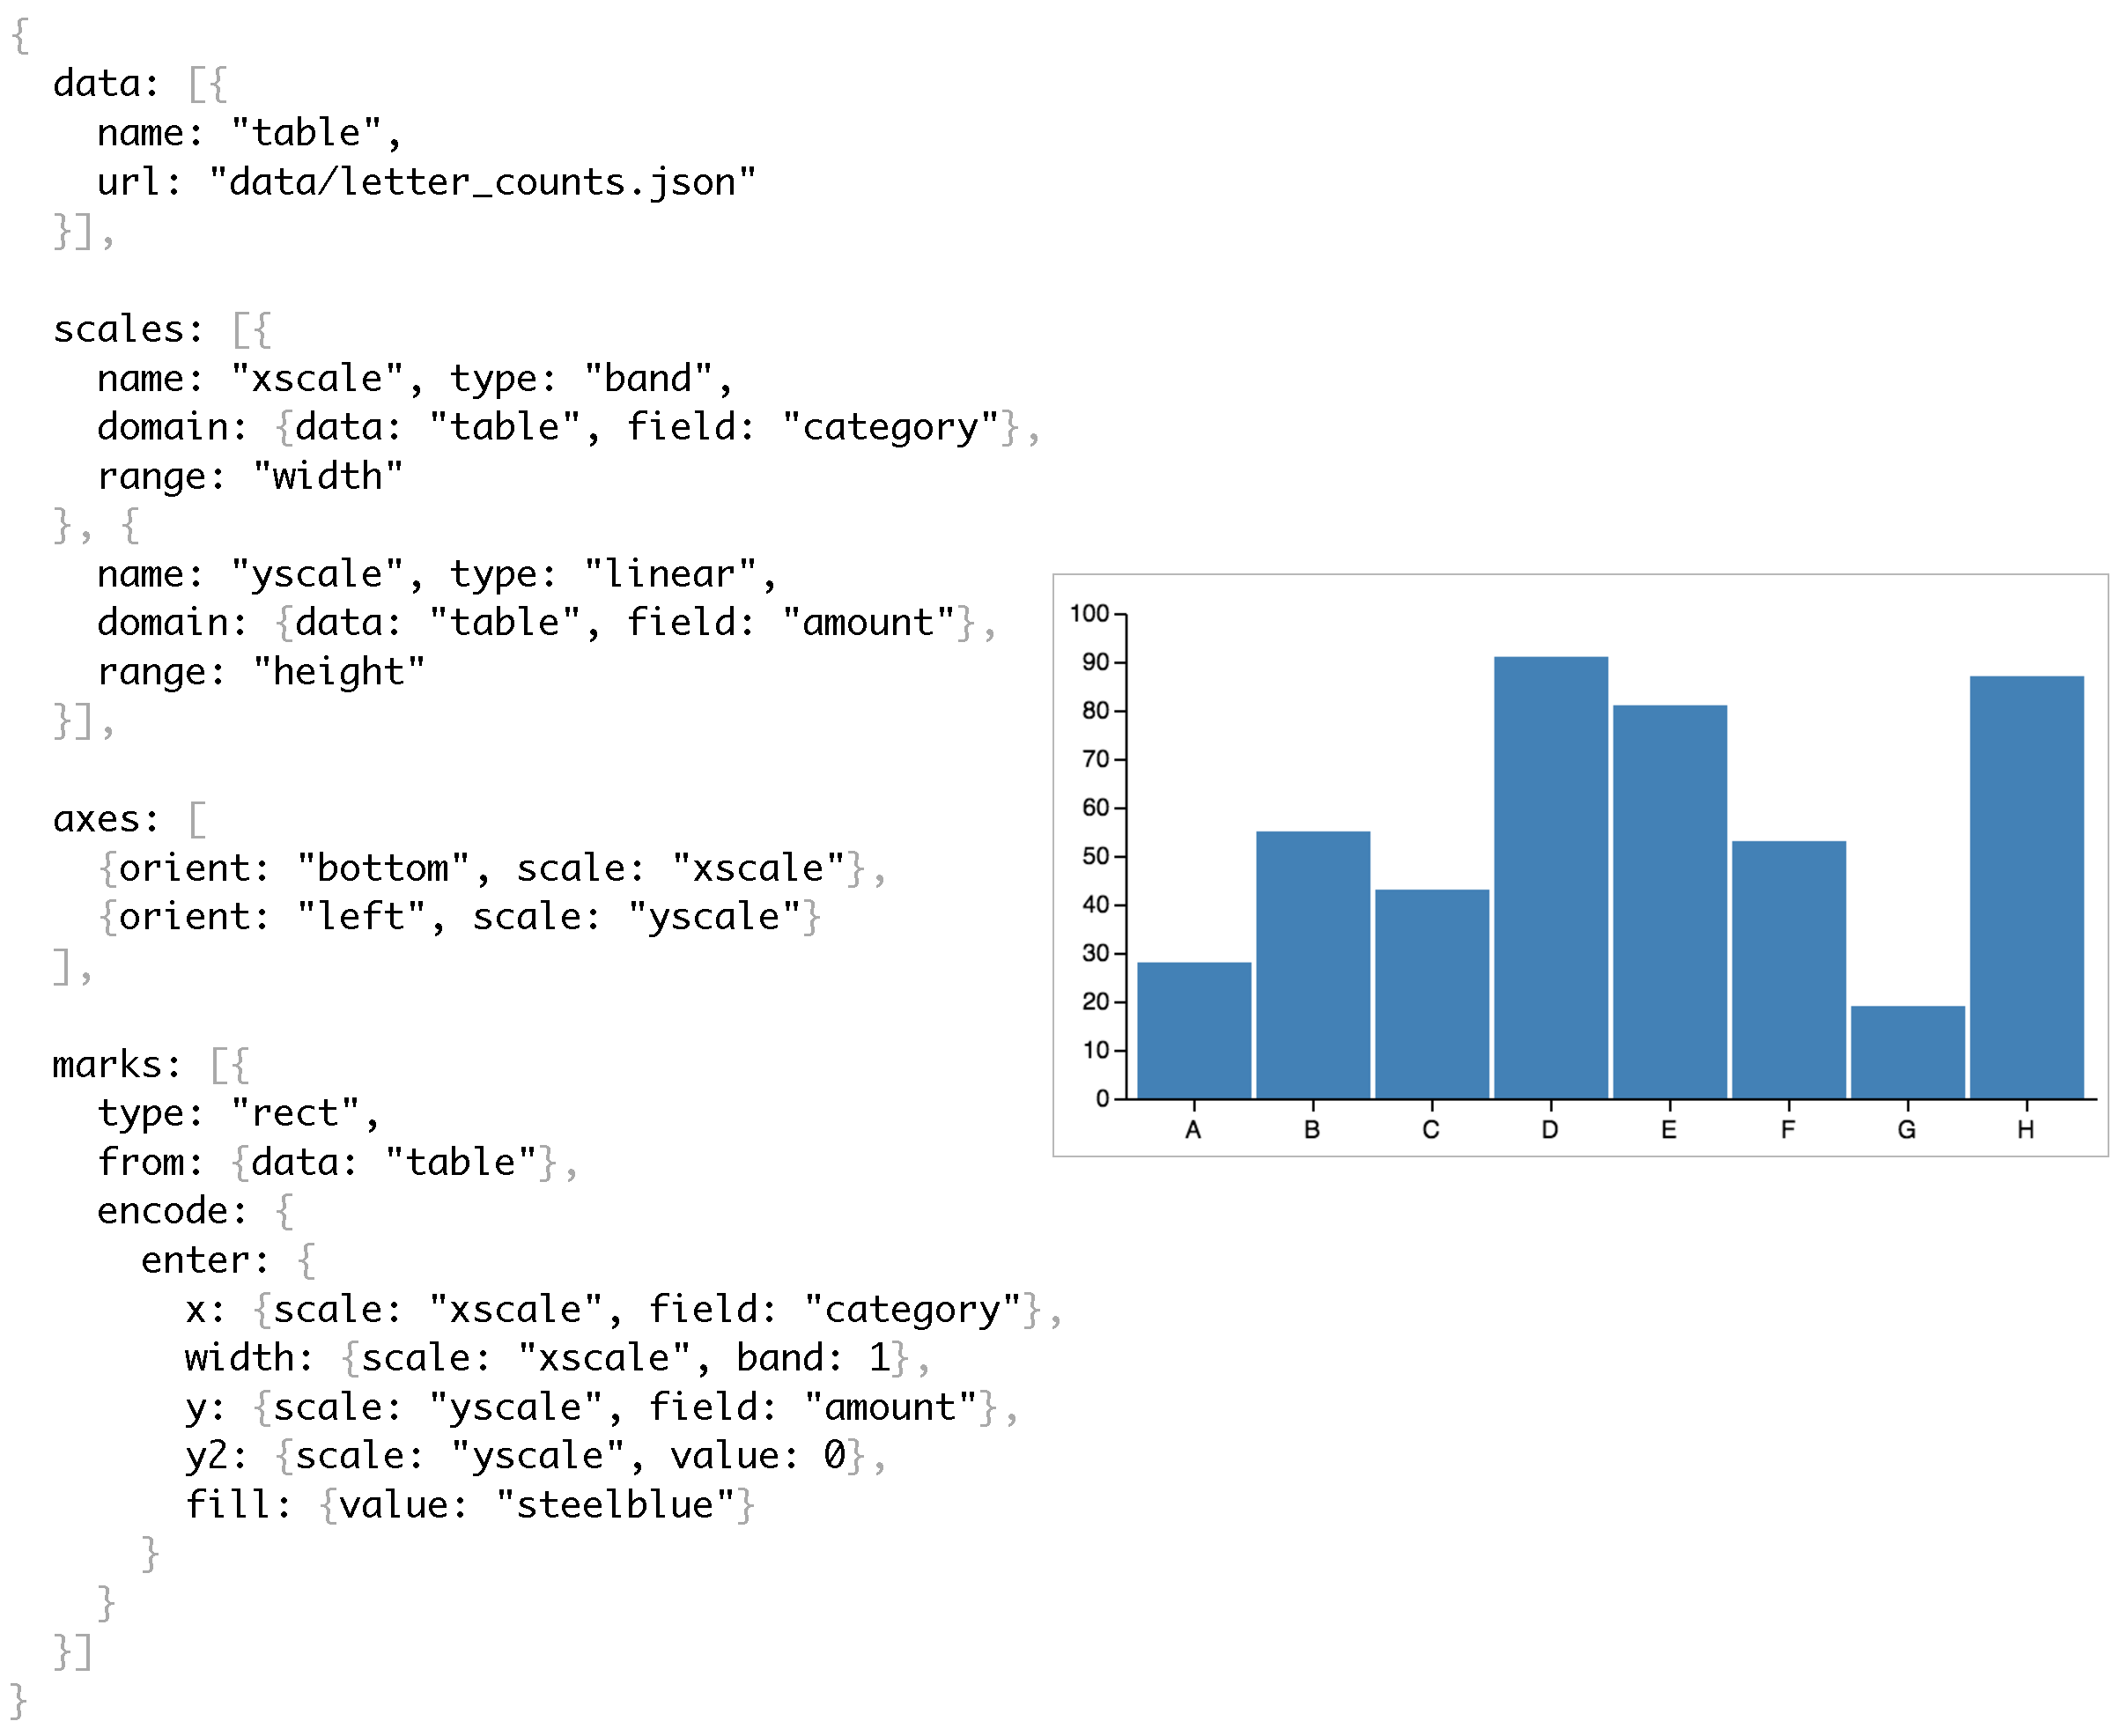
\includegraphics[width=\columnwidth]{barChart}
  \caption{A JSON specification for a bar chart, demonstrating Vega's
  abstractions for visual encoding. Data is imported from a URL. Scales
  transform data values to visual values. Properties of graphical marks (in
  this case rectangles) are determined by scale mappings. Guides (here, axes)
  can be instantiated as well.}
  \label{fig:vg:barChart}
\end{figure}

In response, Reactive Vega introduces a model for \emph{declarative} interaction
design.

\section{Interaction Language Design}
\label{sec:vg:primitives}

\vspace{-10pt}

Reactive Vega models low-level events as composable data streams from which
higher-level semantic \emph{signals} can be constructed. Signals feed
\emph{predicates} and \emph{scale inversions}, to generalize interactive
selections at the level of item geometry (pixels) into interactive queries over
the data domain. \emph{Production rules} then use these queries to manipulate
the visualization's appearance. To facilitate reuse and sharing, these
constructs can be encapsulated as named \emph{interactors}: standalone, purely
declarative specifications of interaction techniques.

\vspace{-10pt}

\subsection{Event Streams and Signals}
\label{sec:vg:events}

\vspace{-10pt}

Reactive Vega adapts the semantics of Event-Driven Functional Reactive
Programming~\cite{wan:efrp}. Low-level input events (e.g., mouse events) are
captured as time-varying \emph{data streams}, rather than event callbacks. This
abstraction reduces the burden of composing and sequencing
events\,---\,operations that would require several callbacks and some external
state under an imperative paradigm. To this end, we introduce a syntax for
specifying event streams (\cref{fig:vg:eventStreams}). While prior work has
formulated regex-based symbols for event selection~\cite{kin:proton++} we
believe our approach, by mimicking CSS selectors, will be more familiar to
designers.

\begin{figure}[b!]
  \centering
  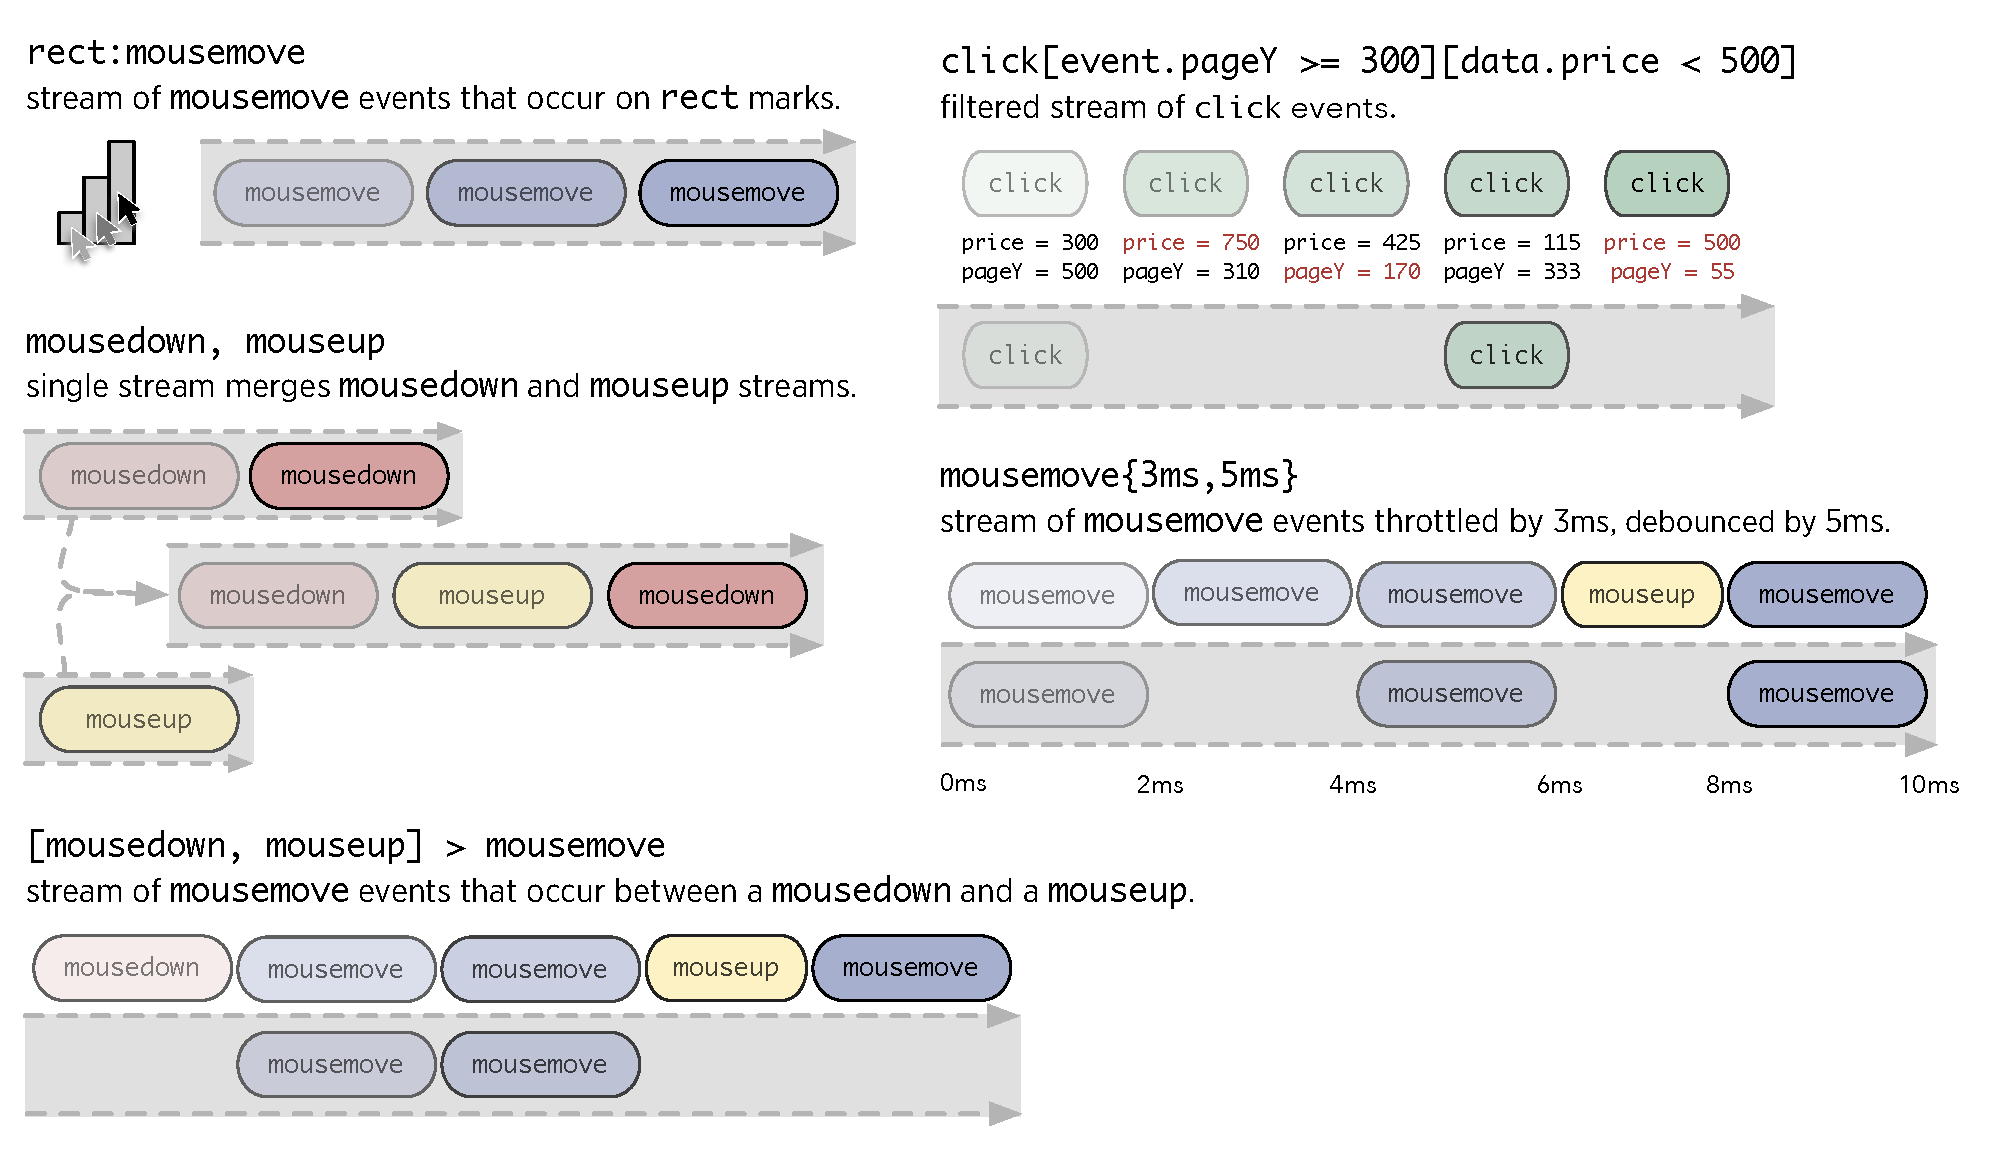
\includegraphics[width=\columnwidth]{eventStreams}
  \caption{Reactive Vega provides an event stream selector syntax, inspired by
  CSS selectors, to compose, filter, and sequence input events.}
  \label{fig:vg:eventStreams}
\end{figure}

A basic event stream selector is specified by a particular event type (e.g.,
\texttt{mousemove}), optionally prepended with the source of the
events\,---\,either a mark type (e.g., \texttt{rect:}) or name (e.g.,
\texttt{@cell:}). The comma operator (\texttt{,}) merges streams to produce a
single stream with interleaved events. Square brackets (\texttt{[]}) filter
events based on their properties. When followed by the right-combinator
(\texttt{>}), the brackets indicate a ``between filter,'' defining bounding
events for the stream. For instance, \texttt{[mousedown, mouseup] > mousemove}
captures \texttt{mousemove} events that occur between a \texttt{mousedown} and
\texttt{mouseup} (i.e., ``drag'' events). To throttle or debounce an event
stream, timing information can be specified between curly braces (e.g.,
\texttt{\{100, 200\}} throttles a stream by 100ms and debounces it by 200ms).
All operators are composable. For instance, \texttt{[mousedown[event.shiftKey],
window:mouseup] > window:mousemove\{100, 200\}} specifies a stream of throttled
and debounced drag events that are only triggered when the shift key is pressed.

With Reactive Vega, interaction events are a first-class data source. They can
be run through the full gamut of data transformations and can drive visual
encoding primitives. While doing so can usefully visualize a user's interaction,
for added expressivity, event streams can also be composed into reactive
expressions called \emph{signals}. By default, signals are evaluated using the
most recent event from a stream. However, signals can also define finite-state
machines by drawing from multiple streams\,---\,each stream triggers a state
transition.

Signals can be used to directly specify visual encoding primitives (e.g., a
mark's fill color) thereby endowing them with reactive semantics. When an event
fires, it enters appropriate streams and is propagated to corresponding signals;
signals are re-evaluated and dependent visual encodings re-rendered
automatically.

Upon definition, signals must be given unique names. These named entities are
then used to define the rest of an interaction technique, thereby decoupling
input events from downstream application logic. Thus, an interaction can be
triggered by a different set of events by simply rebinding signal declarations.
As we later demonstrate, rebinding is particularly useful for retargeting
interactions or for combining otherwise conflicting interactions.

\vspace{-10pt}

\subsection{Predicates and Scale Inversion}

\vspace{-10pt}

Selection is a fundamental operation in interactive visualization design~
\cite{heer:generalized}. Once a selection is made, subsequent operators can be
applied to manipulate the selected items. For visual design, it can be
sufficient to make a predetermined selection (e.g., ``select all rectangles'').
With interaction design, however, selections are driven by user
input\,---\,brushing over points of interest, or adjusting a slider to filter
data.

\begin{figure}[t!]
  \centering
  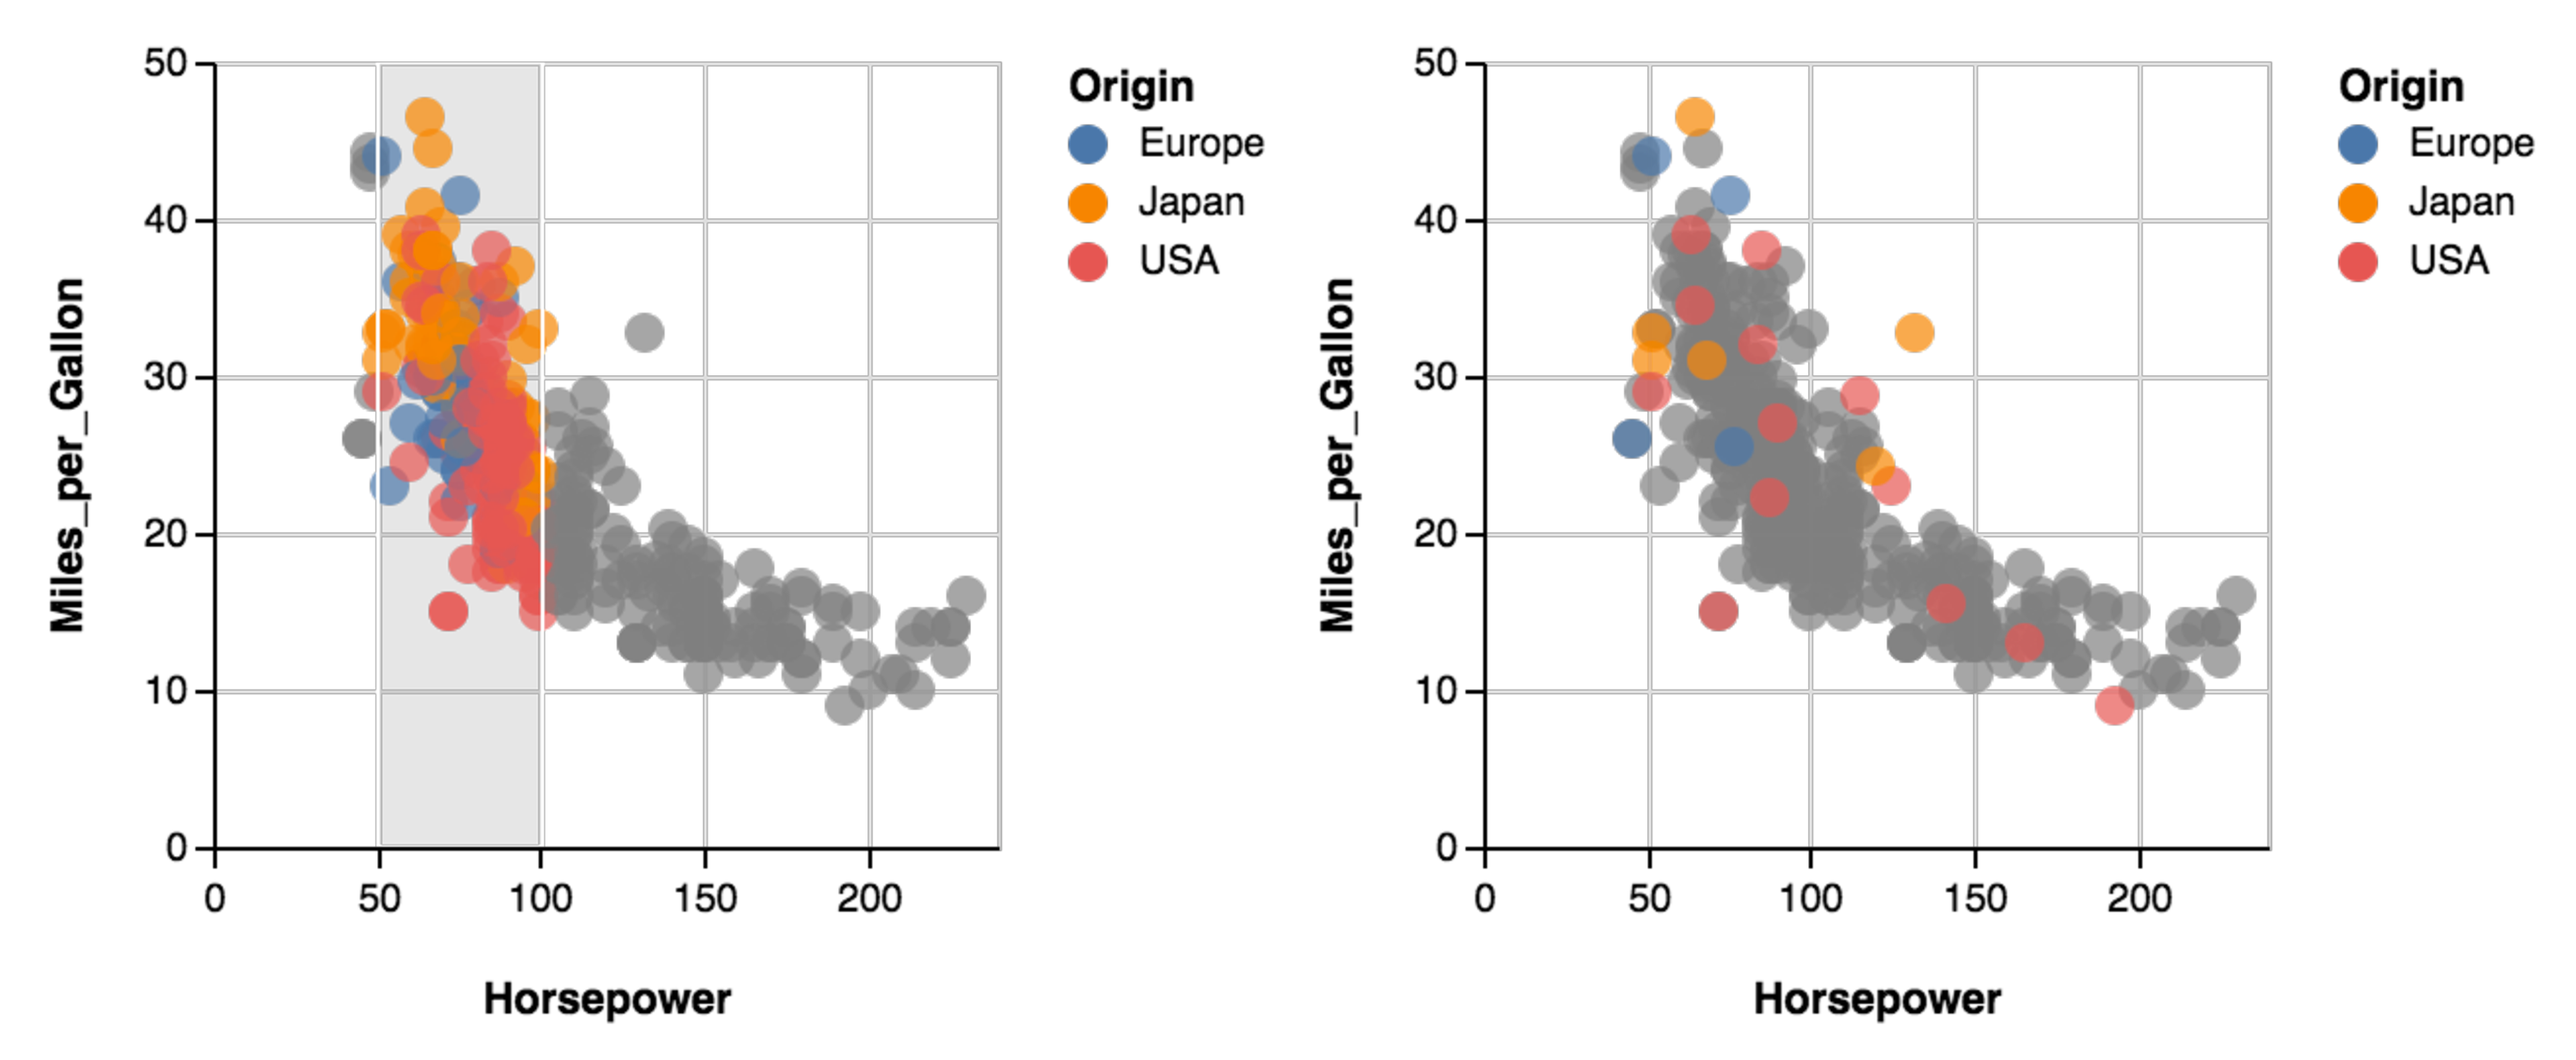
\includegraphics[width=0.9\columnwidth]{predicates}
  \caption{Points are highlighted using (left) an intensional predicate
  \texttt{50 $\leq$ Horsepower $\leq$ 100} or (right) an extensional predicate
  with members \texttt{\#56, \#110, \#79, \#95, \#40, \#120, ...}.}
  \label{fig:vg:predicates}
\end{figure}

To express interactive selections, we introduce reactive \emph{predicates}. As
shown in \cref{fig:vg:predicates}, predicates can be constructed either with an
\emph{intensional} definition\,---\,specifying conditions over properties of
selected members\,---\,or an \emph{extensional} one\,---\,explicitly enumerating
all members of a selection.

Predicate operands are typically signals and, as signals drawn from input event
streams, predicates express interactive selections at the visual (or pixel)
level by default. However, pixel-level selection is often insufficient. A single
visualization may have multiple distinct visual spaces, or an interactive
technique may wish to coordinate several visualizations. In such cases, it is
necessary to generalize an interactive selection into a query over the data
domain~\cite{heer:generalized}. Scale functions are a critical component in
visualization design~ \cite{wilkinson:grammar} as they transform data values
into visual values such as pixels or colors. By applying an \emph{inverted}
scale function to predicate operands, we can lift a predicate to the data
domain. \Cref{fig:vg:scaleInversion} demonstrates how a predicate defines an
interactive selection and, when coupled with scale inversions, an interactive
query to drive an overview\,+\,detail visualization.

\newpage
\begin{figure}[h!]
  \centering
  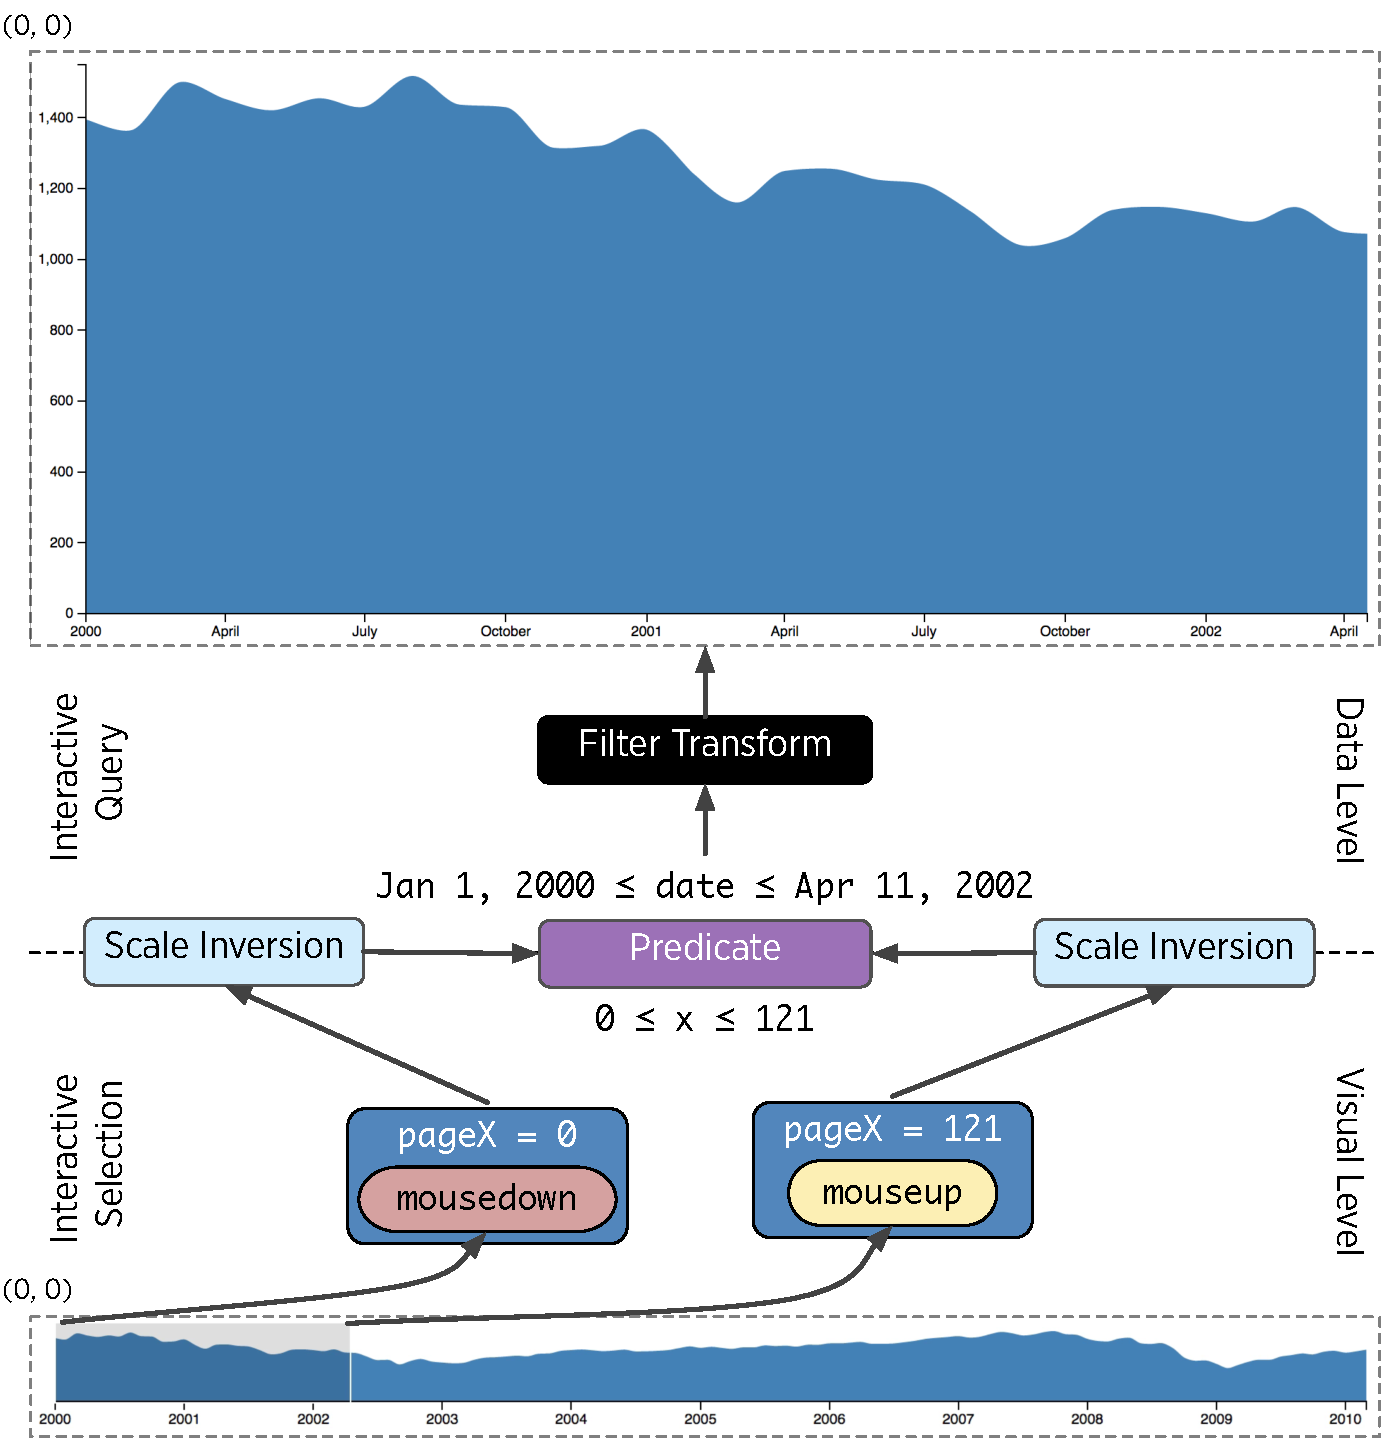
\includegraphics[width=\columnwidth]{scaleInversion}
  \caption{\emph{Predicates} use signal values to define interactive selections
of elements. Using \emph{scale inversions}, predicates can be generalized to
define interactive queries, and thus operate across different coordinate spaces:
overview (bottom) and detail (top).}
  \label{fig:vg:scaleInversion}
\end{figure}


\subsection{Production Rules}

\vspace{-10pt}

Production rules are an established design pattern for visualization
specification~\cite{heer:designpatterns} that we endow with reactive semantics.
A rule defines the outcome of evaluating an \texttt{if-then-else} chain to set
property values. For example, a rule might set a mark's fill color using
scale-transformed data if predicate \texttt{A} is true, set it to yellow is
predicate \texttt{B} is true, or otherwise set the color to grey by default.

\vspace{-10pt}

\subsection{User-Defined Functions}
\label{sec:udfs}

\vspace{-10pt}

During our design process, we encountered visualizations in which interactions
trigger custom data transforms. For example, sorting a co-occurrence matrix by
frequency or querying time-series data via relaxed
selections~\cite{holz:relaxed}. It is not feasible for a declarative language to
natively support all possible functions, yet custom operations must still be
expressible. Following the precedent of languages such as SQL, we provide
\emph{user-defined functions}. Such functions must be defined and registered
with the system at runtime, and can subsequently be invoked declaratively within
the specification. User-defined functions ensure that the language remains
concise and domain-specific, while ensuring extensibility to idiosyncratic
operations.

\vspace{-10pt}

\subsection{Encapsulated Interactors}

\vspace{-10pt}

To enable reuse of custom interaction techniques, Reactive Vega's interaction
primitives can be parameterized and encapsulated as named \emph{interactors}.
Inspired by Garnet's component of the same name~\cite{myers:garnet}, a Reactive
Vega's interactor can subsequently be applied to a visualization and functions
as a mixin. Its specification is merged into the host's and, to prevent
conflicts, its components are addressable only under its namespace.
\Cref{fig:vg:splomInteractor,fig:vg:brush} illustrate how a brushing
interaction (within a single scatterplot) can be extracted to a standalone
interactor, and reapplied to brush \& link a scatterplot matrix.
% !TEX root = ../thesis.tex
\section{Example Interactive Visualizations}
\label{sec:vg:examples}

\vspace{-10pt}

To evaluate the expressivity of our language, we present a range of examples and
demonstrate coverage over Yi~et~al.'s interaction
taxonomy~\cite{yi:understanding}. Yi~et~al. identify seven categories based on
user intent: \emph{select}, to mark items of interest; \emph{connect}, to show
related items; \emph{abstract/elaborate}, to show more or less detail;
\emph{explore}, to examine a different subset of data; \emph{reconfigure}, to
show a different arrangement of data; \emph{filter}, to show something
conditionally; and, \emph{encode}, to use a different visual encoding. It is
important to note that these categories are not mutually exclusive, and an
interaction technique can be classified under several categories. We choose
example interactive visualizations to demonstrate that our model can express
interactions across all seven categories and how, through composition of its
primitives, supports the accretive design of richer interactions.

\begin{figure}[h!]
  \centering
  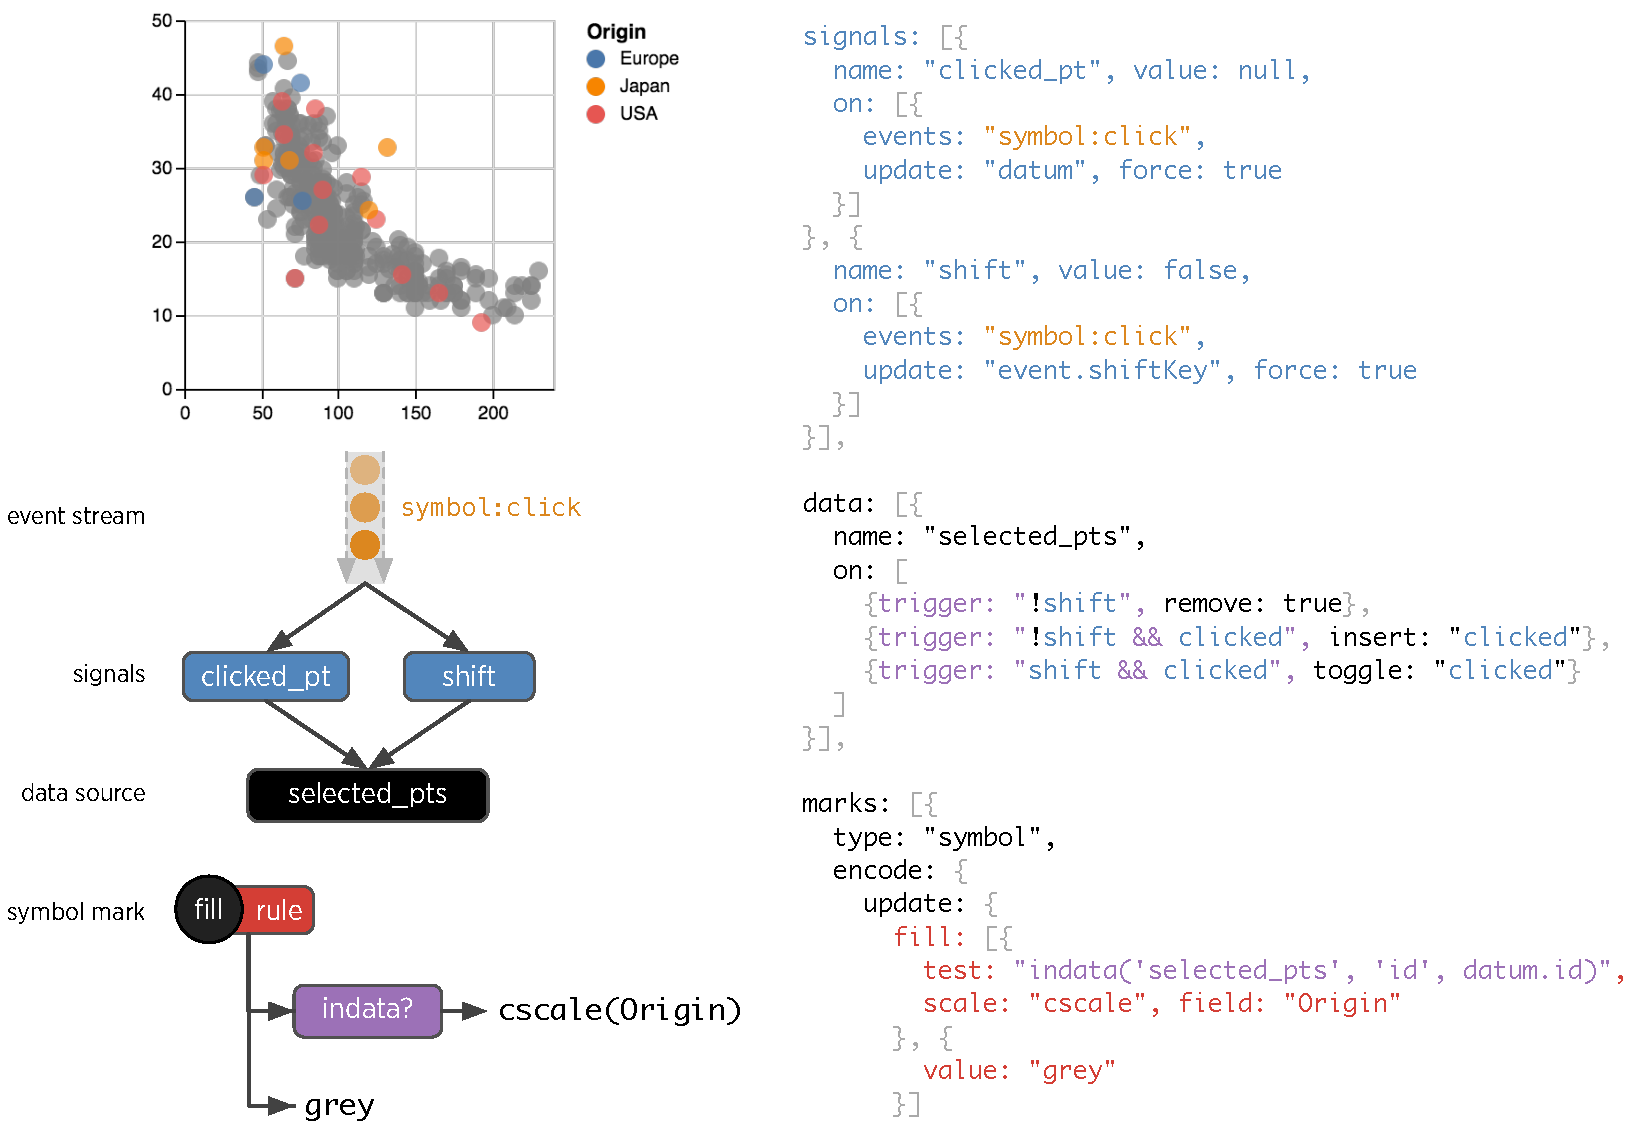
\includegraphics[width=\columnwidth]{shiftClick}
  \caption{Reactive Vega \textsc{json} for a click-to-highlight interaction.
  Signals over a click stream feed data transform to toggle values in a data
  source. A production rule uses a predicate to set marks' fill color.}
  \label{fig:vg:shiftClick}
\end{figure}

\subsection{Selection: Click/Shift-Click and Brushing}

\vspace{-7pt}

\Cref{fig:vg:shiftClick} provides a snippet of Reactive Vega \textsc{json} for a
click-to-highlight interaction. Signals constructed over a click stream feed
data transforms that toggle values in the \texttt{selected\_pts} data source. An
intensional predicate tests for the shift key. If it is not pressed, the data
source is cleared prior to inserting the clicked values. A production rule sets
the fill color of selected points using an extensional predicate.

Similarly, \cref{fig:vg:brush} demonstrates the Reactive Vega \textsc{json}
necessary to enable brush selections. Signals are registered to capture the
start and end positions of the brush, by default \texttt{mousedown} and
\texttt{[mousedown, mouseup] > mousemove}, respectively. Scale inversions are
invoked to calculate the data extents of the brush, which are used to define an
intensional predicate to express the brushed data range. As before, the
predicate is used within a production rule to set the fill color of selected
points.

\begin{figure}[h!]
  \centering
  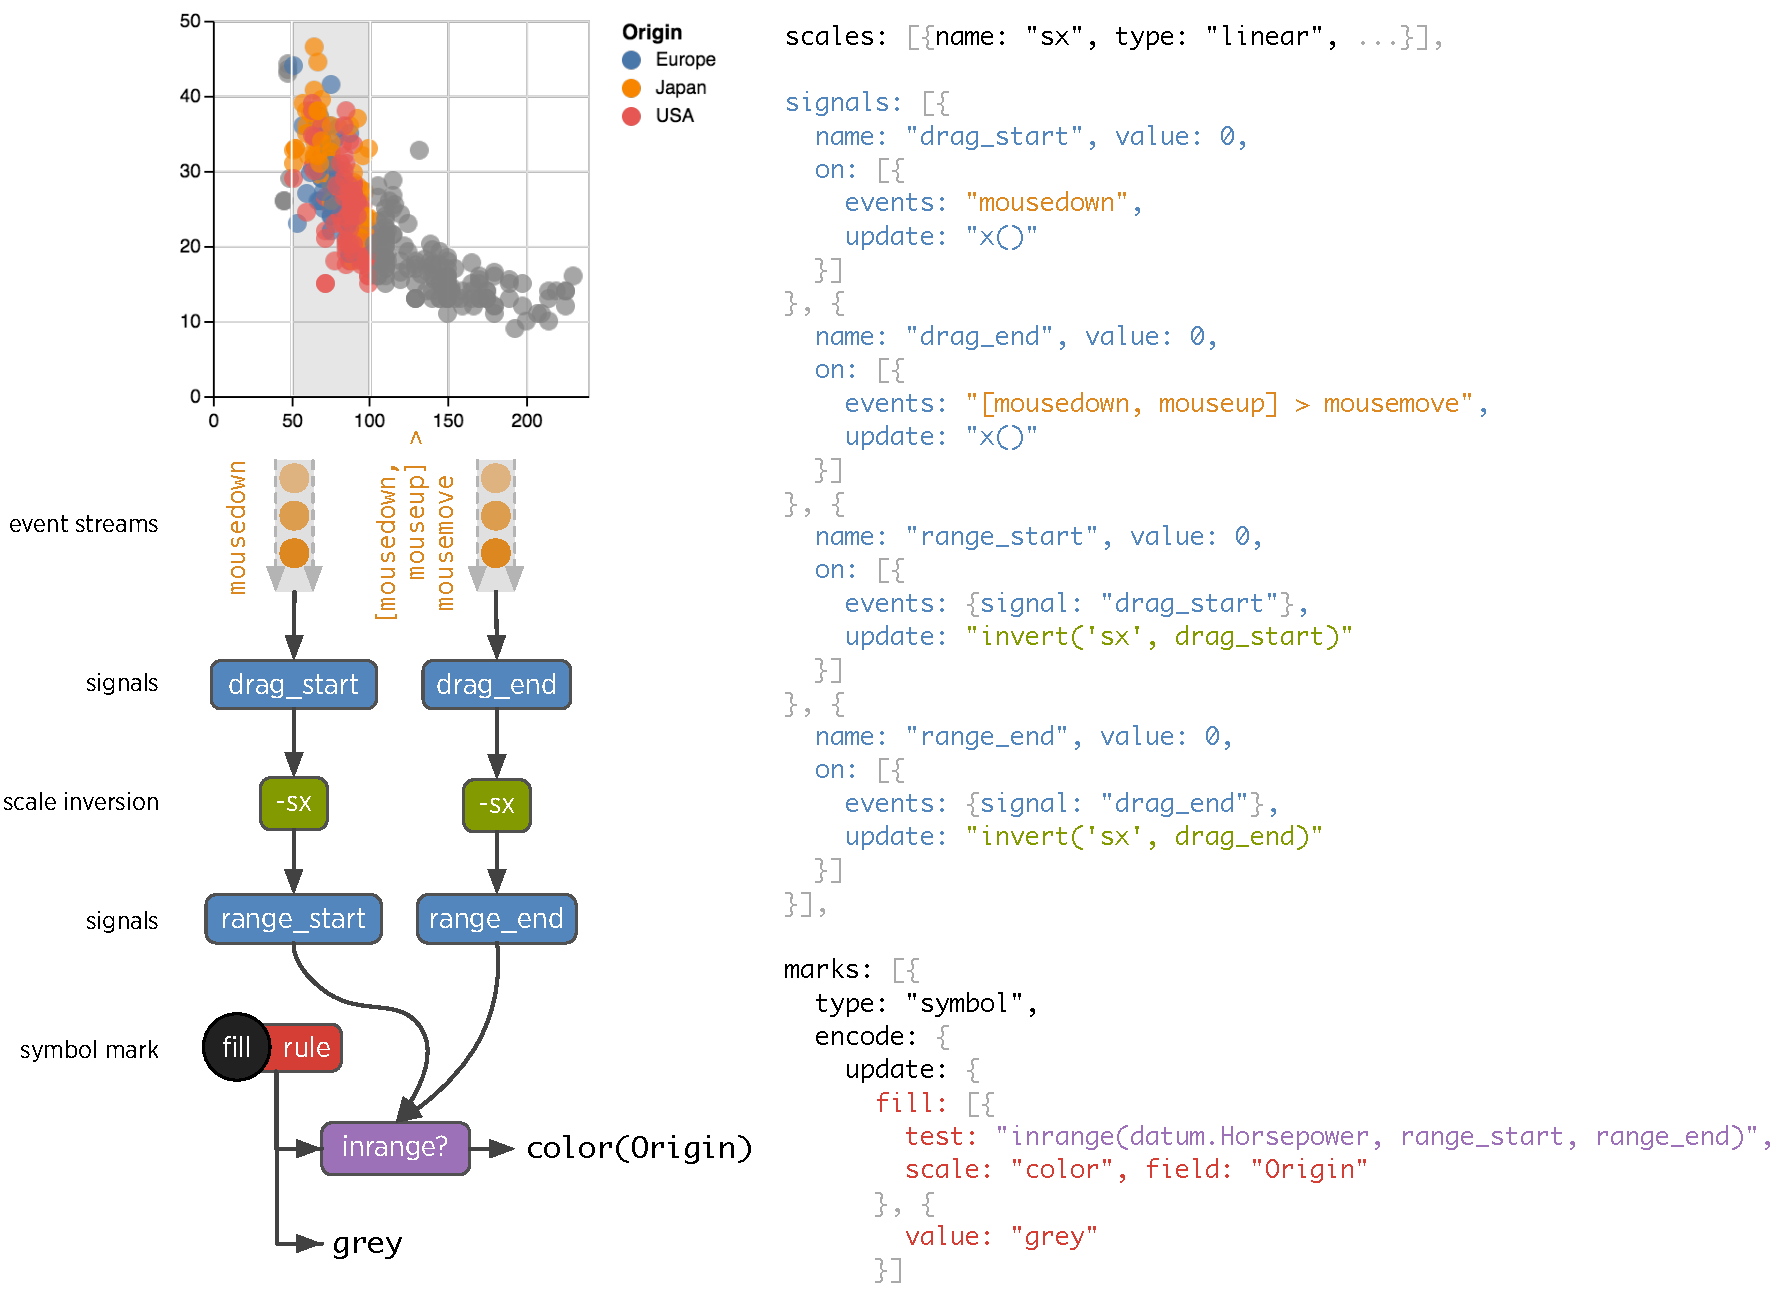
\includegraphics[width=0.91\columnwidth]{brush}
  \caption{A \textsc{json} snippet for one-dimensional brushing. Signals over
  drag events are inverted through the x-scale to construct a data query over
  the \texttt{Horsepower} field.}
  \label{fig:vg:brush}
\end{figure}

\begin{figure}[h!]
  \centering
  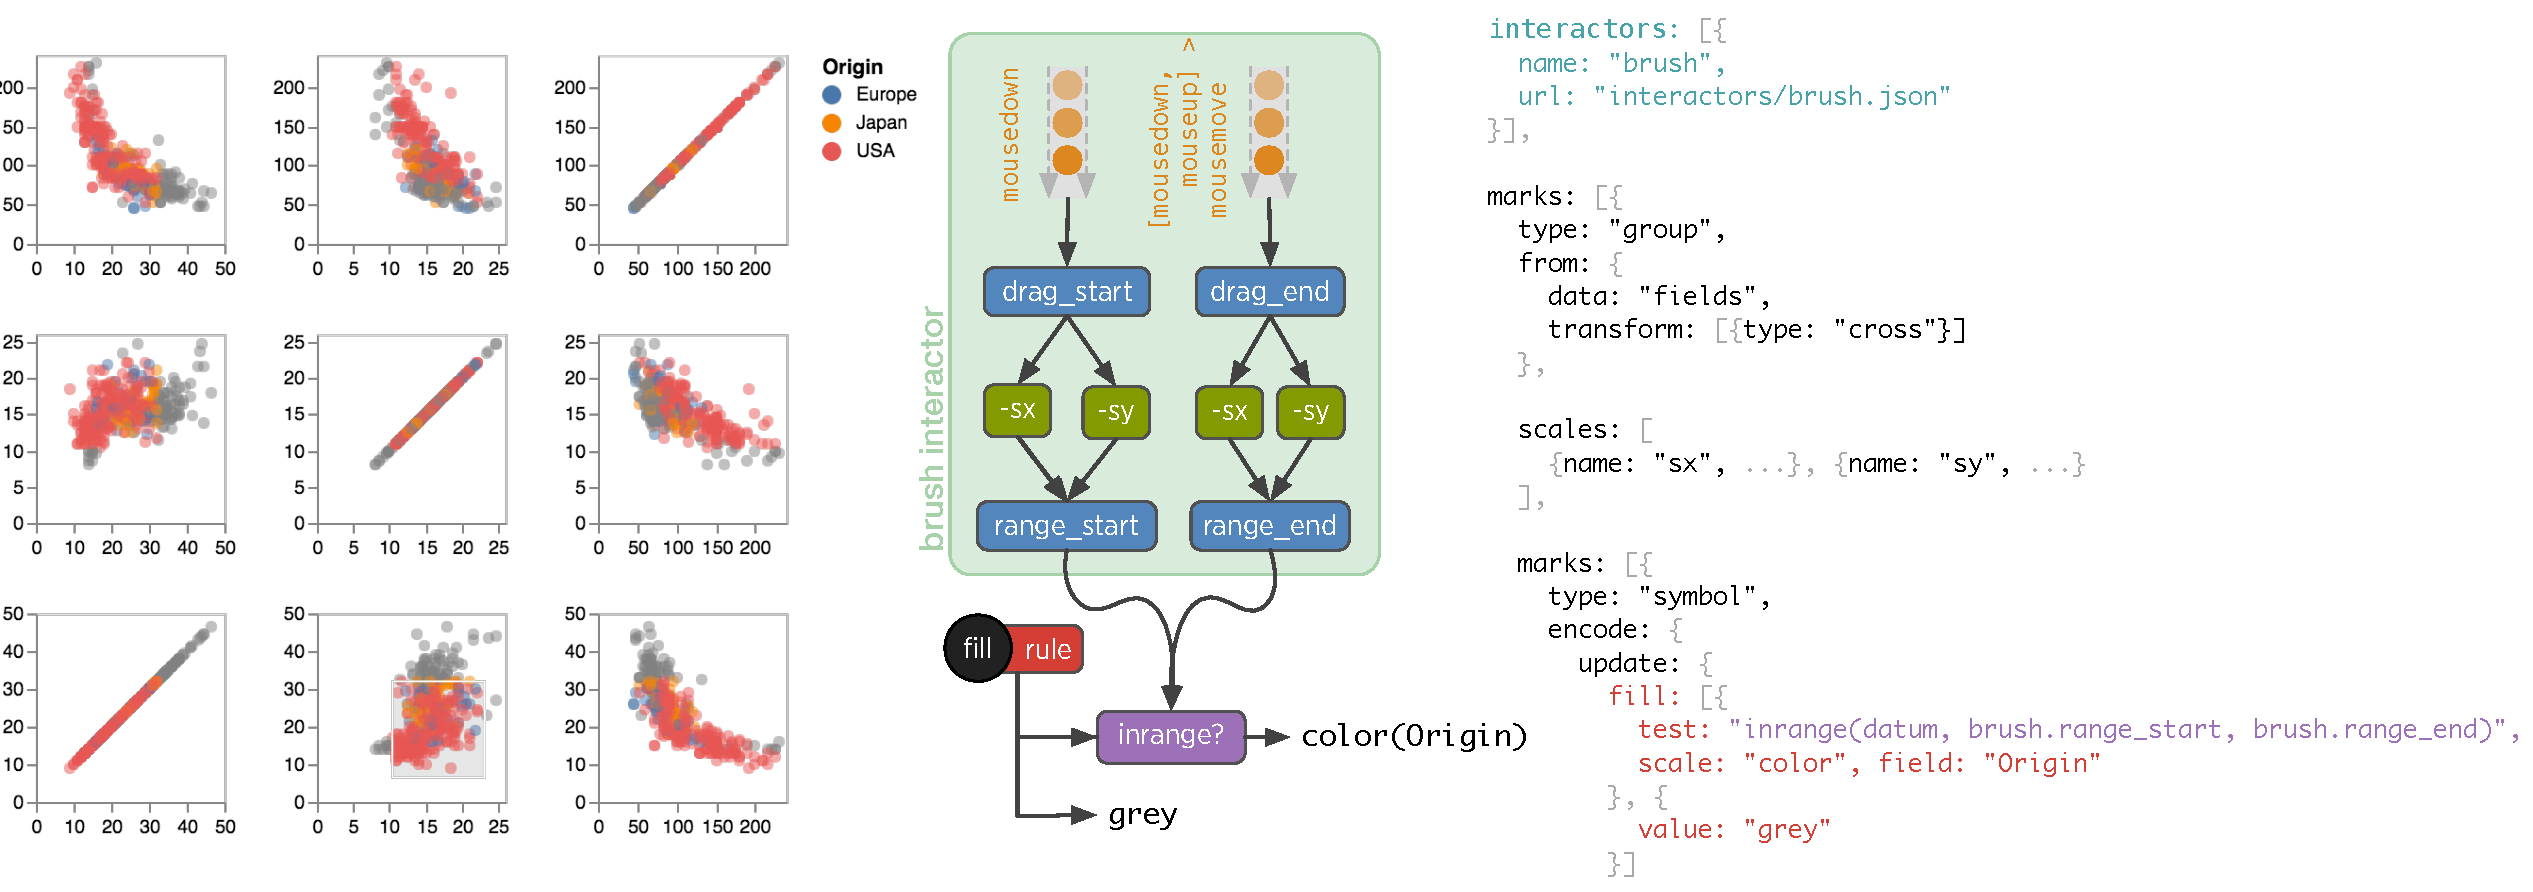
\includegraphics[width=\columnwidth]{splomInteractor}
  \caption{We can extract the brushing interaction from \cref{fig:vg:brush}
  into a standalone interactor, and reapply it to a scatterplot matrix to
  perform brushing \& linking.}
  \label{fig:vg:splomInteractor}
\end{figure}

\subsection{Connect: Brushing \& Linking}

\vspace{-7pt}

\begin{wrapfigure}{l}{0pt}
  \raisebox{0pt}[\dimexpr\height-0.6\baselineskip\relax]{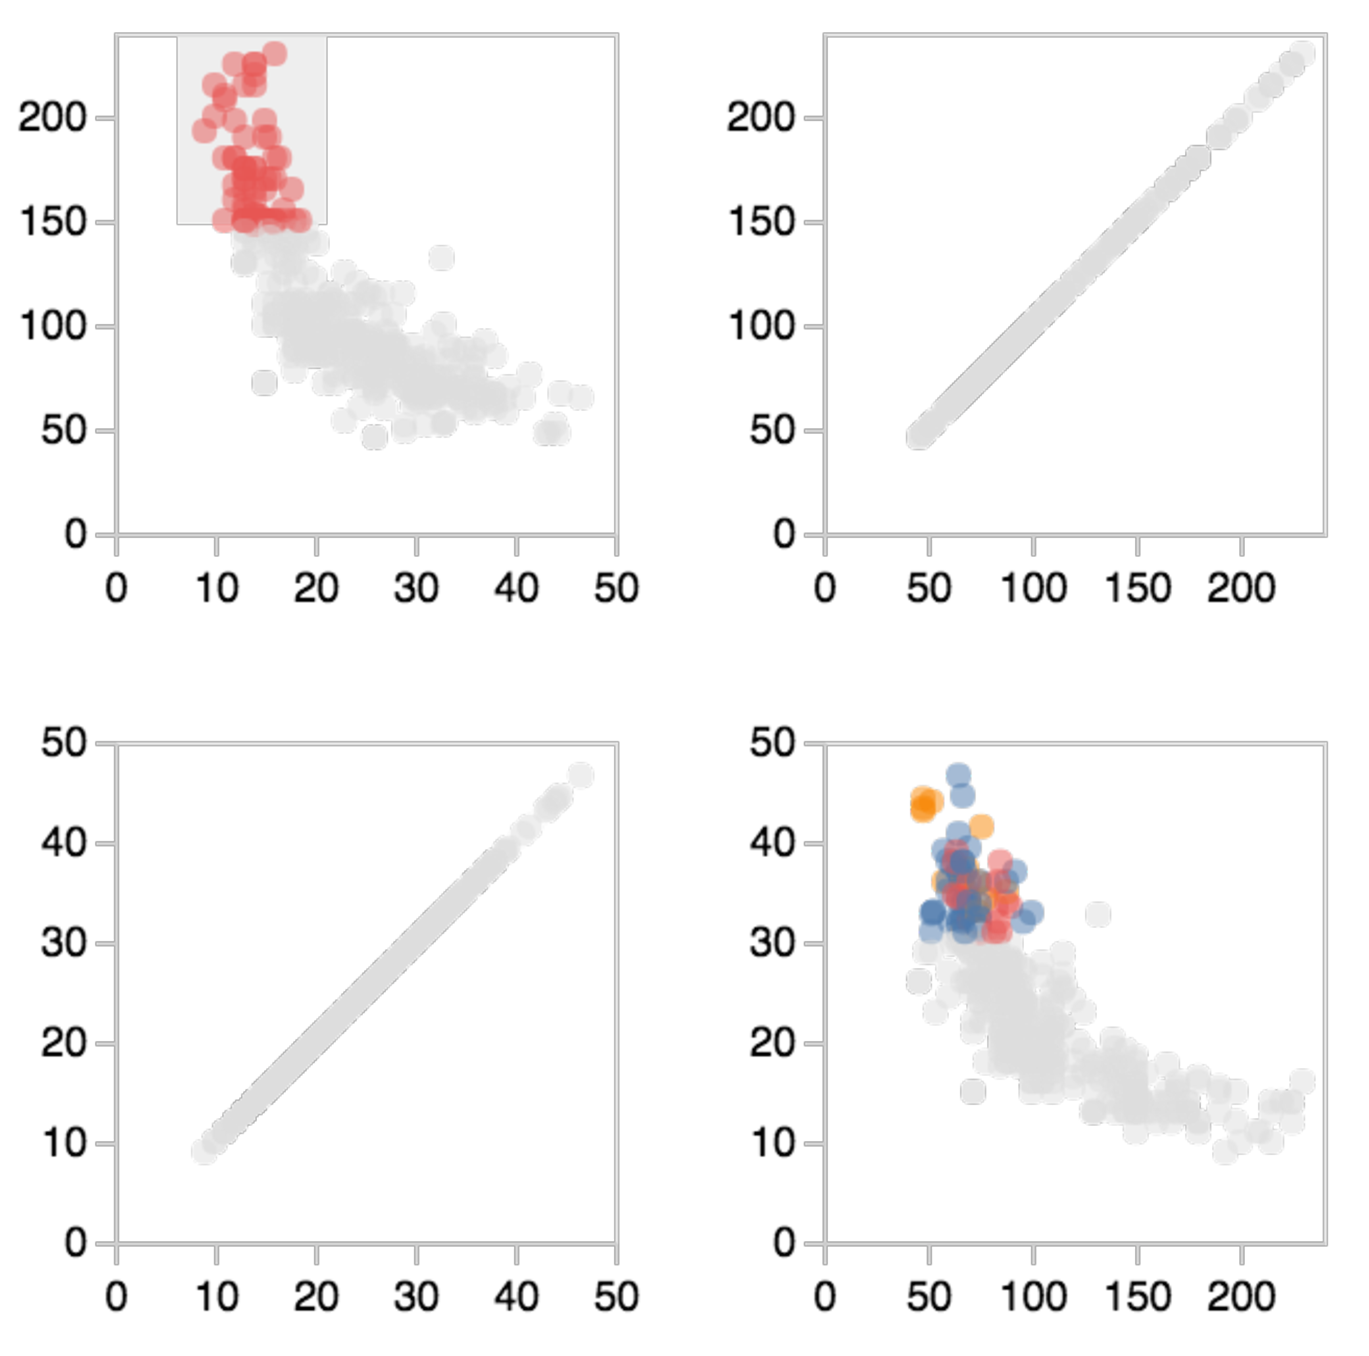
\includegraphics
  [width=0.27\textwidth]{splomPixel}}
\end{wrapfigure}

We can extract the previous interaction into a standalone ``brushing''
interactor, and then apply it to brush \& link a scatterplot matrix as shown in
\cref{fig:vg:splomInteractor}. Each cell of the matrix is an instance of a group
mark with its own coordinate space. The plotting symbol and spatial scale
functions are defined within these groups. Had the interactor's predicates
defined selections over pixel space, the production rule would highlight points
that fall along the same horizontal and vertical pixel regions\,---\,for
example, as shown in the inset figure, brushing over red points would highlight
blue points in the other cells. Instead, the interactor uses scale inversions to
lift the predicate to the data domain, and the production rule correctly links
brushed points across scatterplots.

\vspace{-10pt}

\subsection{Abstract/Elaborate: Overview\,+\,Detail}

\vspace{-7pt}

With our brush interactor, we can also create the overview\,+\,detail
visualization in \cref{fig:vg:scaleInversion}. In this case, brushing is
restricted to the horizontal dimension by overriding the \texttt{height}
property of the interactor's mark, and ignoring the vertical range predicates it
populates. We use the horizontal range predicate with a filter transformation,
to filter points for display in the detail plot. As a user brushes, signals
update the range predicate, which in turn filters points in the data source,
updates scale functions and re-renders the detail view.

\vspace{-10pt}

\subsection{Explore \& Encode: Panning \& Zooming}

\vspace{-7pt}

\begin{figure}[b!]
  \centering
  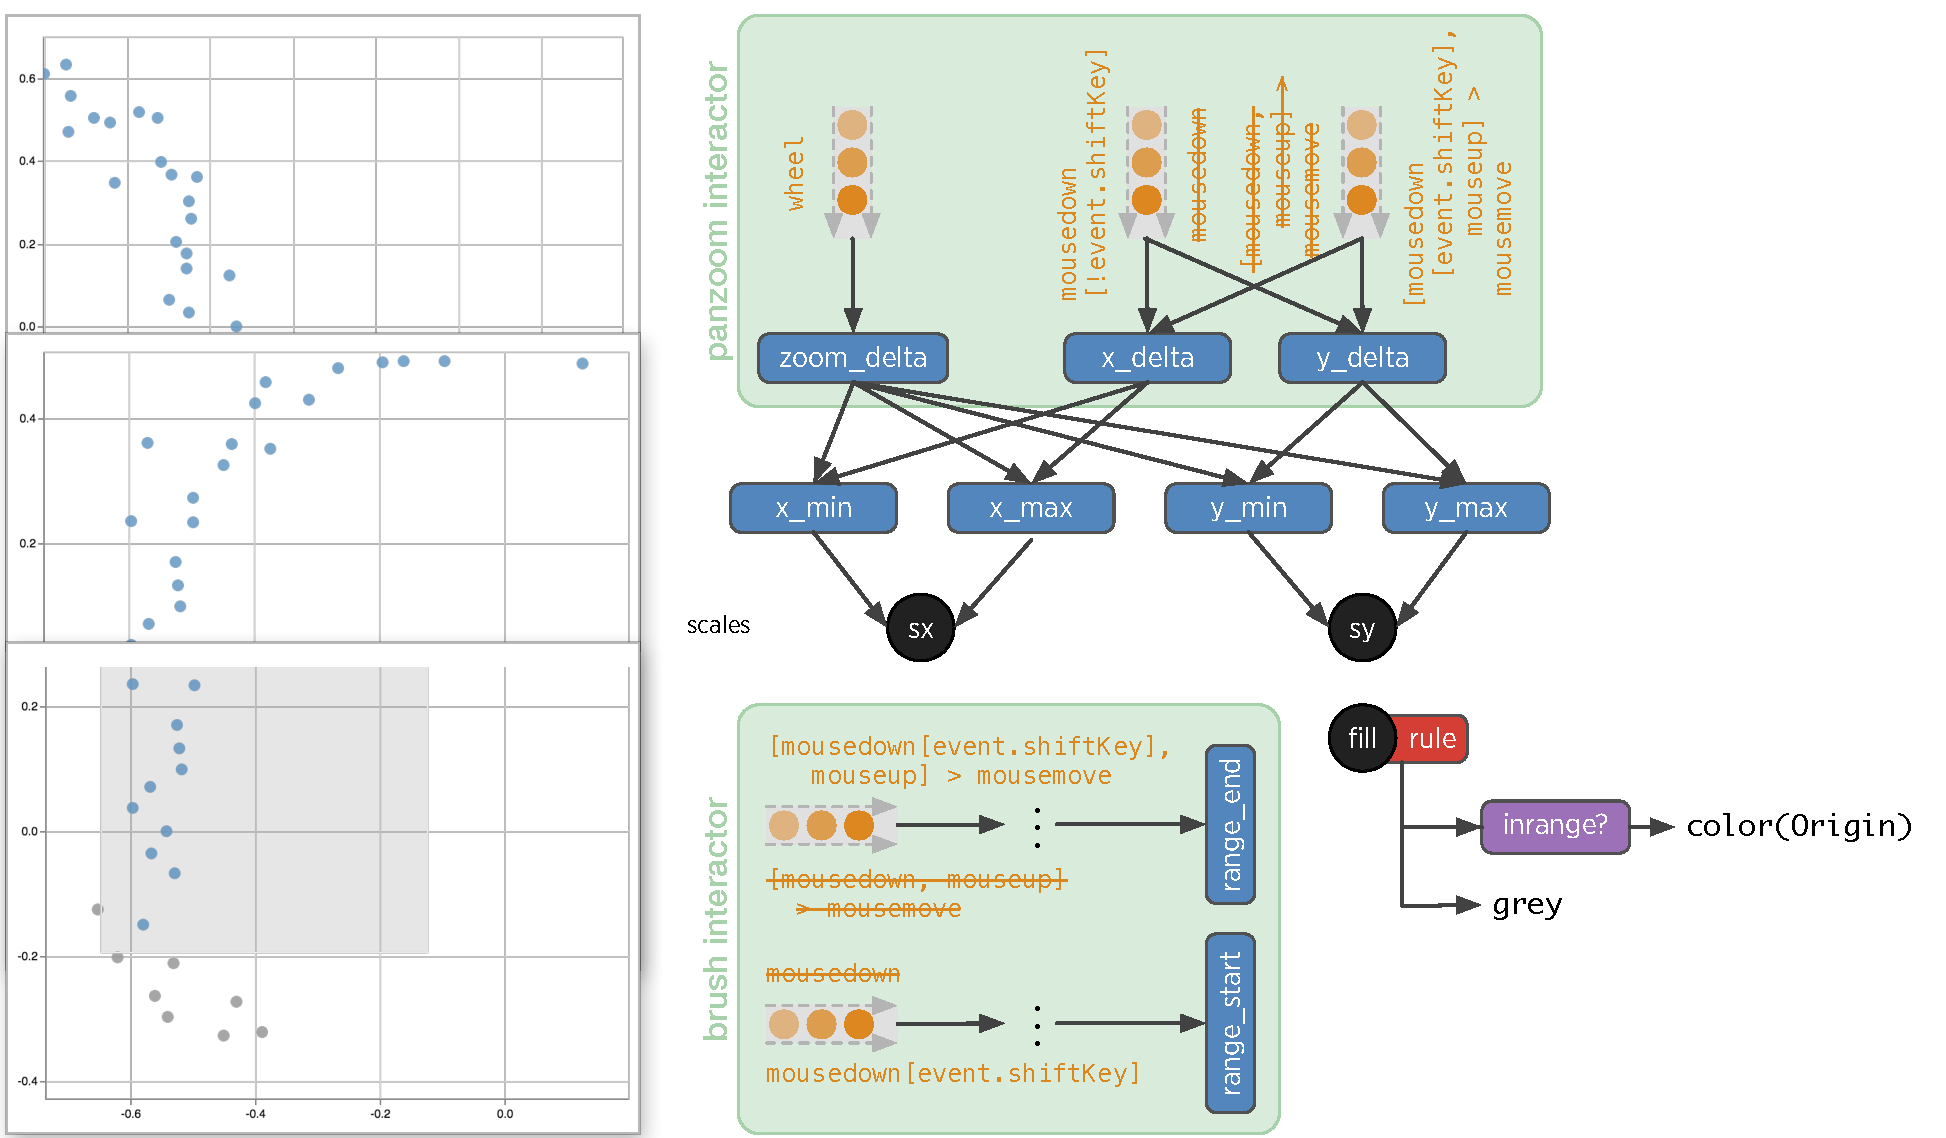
\includegraphics[width=\columnwidth]{panzoom}
  \caption{Panning \& zooming a scatterplot. Brushing is accretively added with
  the brush interactor (\cref{fig:vg:brush,fig:vg:splomInteractor}), and
  conflicts are resolved by rebinding event streams (indicated with
  strikethroughs).}
  \label{fig:vg:panzoom}
\end{figure}

\Cref{fig:vg:panzoom} shows pan and zoom interactions for a scatter plot. By
default, scale functions calculate their domain automatically from a data
source. For this interaction, however, we must parameterize the domain using
reactive signals. For panning, a \texttt{start} signal captures an initial
\texttt{(x,y)} position on \texttt{mousedown}, and subsequent \texttt{pan}
signals calculate a delta on drag (\texttt{[mousedown, mouseup] > mousemove}).
This delta is used to offset the scale domains. Similarly, when \texttt{wheel}
events occur, a \texttt{zoom} signal applies a scale factor to the domains
depending on the zoom direction.

\begin{figure}[b!]
  \centering
  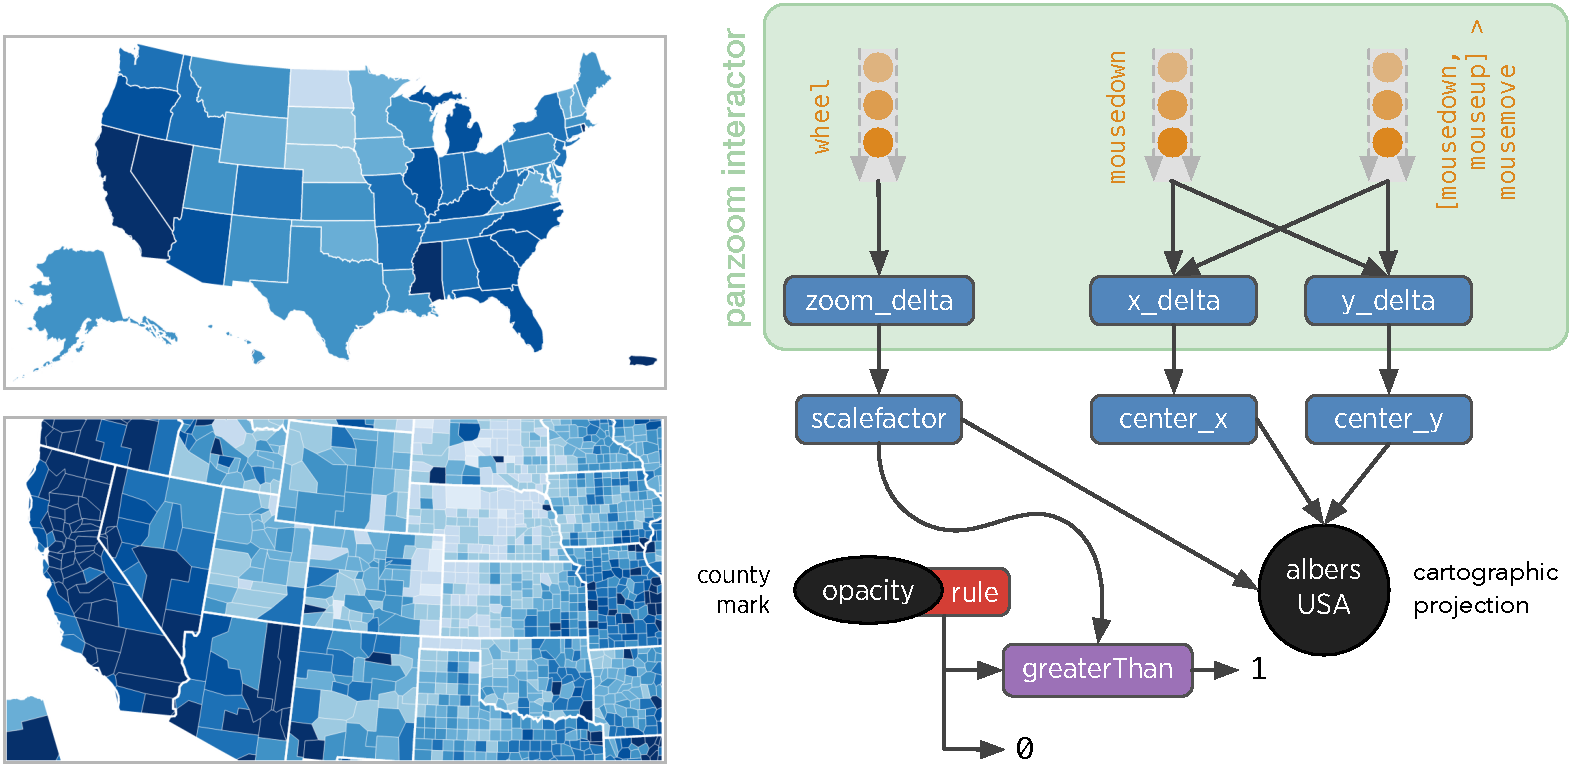
\includegraphics[width=\columnwidth]{semanticZoom}
  \caption{Extracting the pan \& zoom interaction from \cref{fig:vg:panzoom}
  into an interactor, and repurposing it to perform \emph{semantic} zooming on a
  cartographic map. Initially, a choropleth of state-level unemployment in the
  United States is shown. Zooming past a threshold, states break up into
  counties, and show county-level unemployment instead.}
  \label{fig:vg:semanticZoom}
\end{figure}

If we were to also add a brushing interaction to this visualization, a na\"ive
application would yield a conflicting interaction: on drag, both panning and
brushing would occur. One option to resolve this conflict is to begin brushing
only when the shift key is pressed. If we try combining these interactions using
D3~\cite{bostock:d3}, which offers brushing and panning as part of its
interactor typology, specifying this resolution scheme can be onerous.
Additional callbacks must be registered that either instantiate or destroy a
particular interaction depending on the state of the shift key.

With Reactive Vega, the brush and pan signals can be rebound without modifying
the interactor definitions. Instead, we provide alternate source event streams
when instantiating the interactor\,---\,\texttt{mousedown[event.shiftKey]} for
brushing, and\\\texttt{mousedown[!event.shiftKey]} for panning.

Moreover, by extracting panning \& zooming into a standalone interactor, we can
repurpose the behavior to instead trigger semantic zooming~\cite{perlin:pad}, an
\emph{encoding} interaction technique shown in \cref{fig:vg:semanticZoom}. At
the top-level, the visualization shows a choropleth map of state-level
unemployment. After crossing a specified zoom threshold, states subdivide to
show a choropleth map of country-level unemployment. Here, the pan signals drive
the geographic projection's translation and the zoom signals drive the
projection's scale parameter. By default, both maps are drawn with states
overlaying counties. A production rule uses a predicate to test whether the zoom
signal is above a specified threshold; if it is, the state-level map is rendered
transparently, displaying the county-level map underneath it.

\vspace{-10pt}

\subsection{Reconfigure: Index Chart}

\vspace{-7pt}

\begin{figure}[b!]
  \centering
  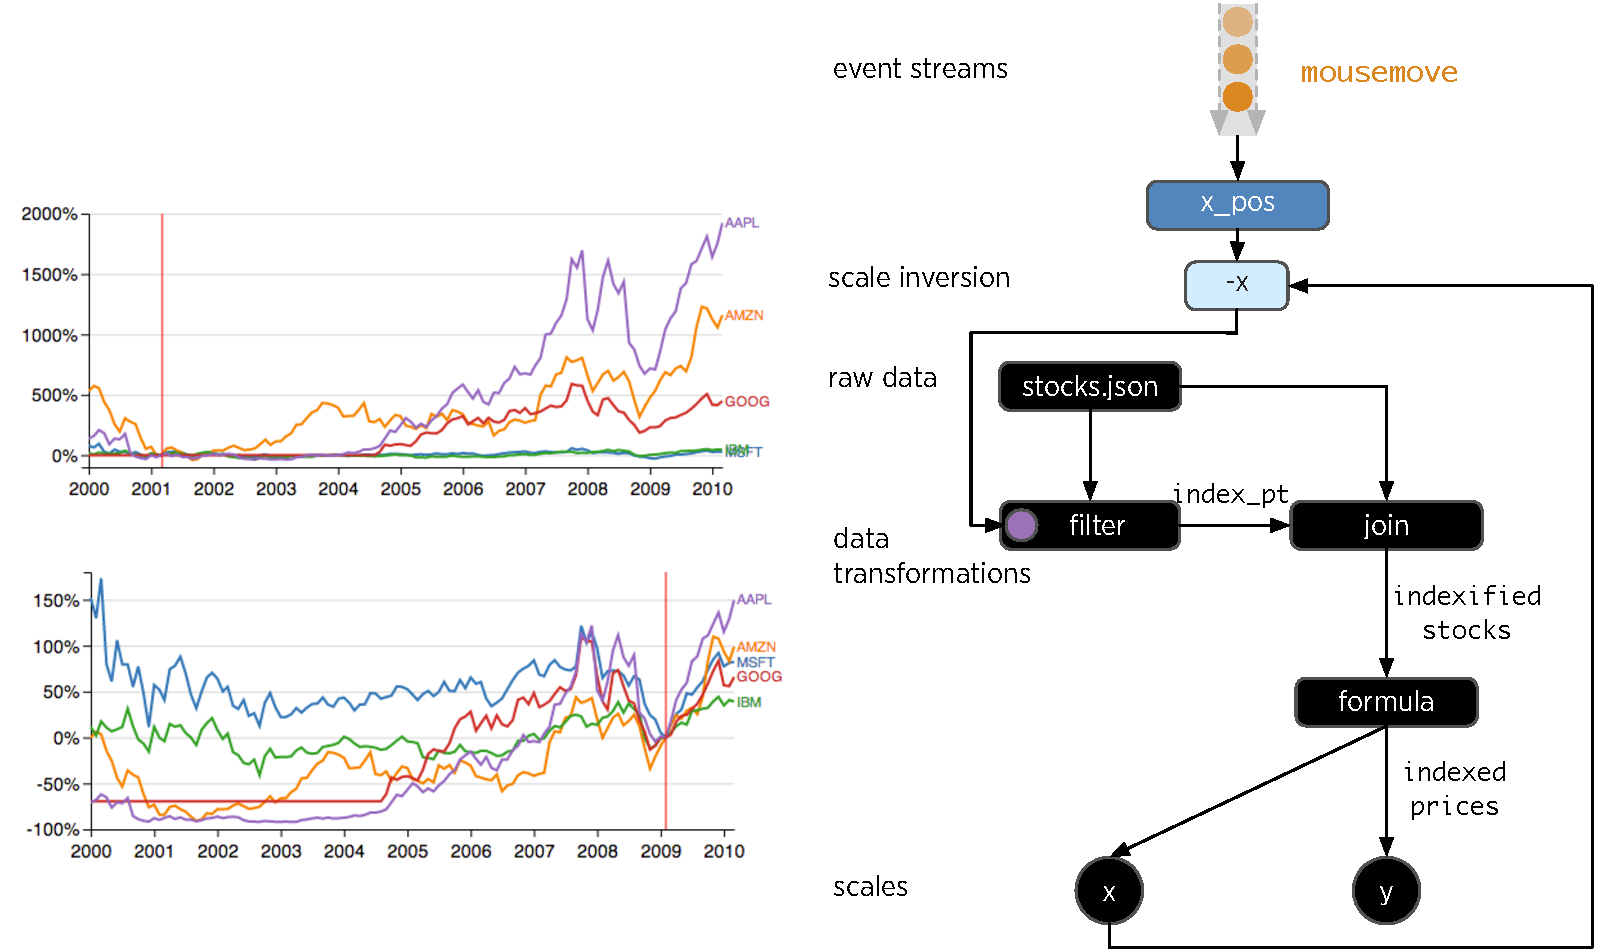
\includegraphics[width=0.89\columnwidth]{indexChart}
  \caption{An index chart shows the percentage changes for time-series data. The
  index point (red vertical line) is determined by the x position of a
  \texttt{mousemove} signal, which filters points using a predicate.}
  \label{fig:vg:indexChart}
\end{figure}

\Cref{fig:vg:indexChart} shows an index chart: a line chart that interactively
normalizes time series to show percentage change based on the current index
point. To calculate the index point, a signal captures the \texttt{x} coordinate
of \texttt{mousemove}events, and drives it through a scale inversion. As it is a
quantitative scale, scale inversion produces a value from a continuous domain
(i.e., any date/time from Jan 1, 2000--Dec 31, 2010). However, our dataset only
contains stock prices for the start of every month. We use a predicate to ``snap
to'' the closest value for each time series, and use this as our index point.
Using Vega's data transformations, we join the index point against the original
data set and normalize the data values. Scale functions are defined in terms of
the normalized data.

\vspace{-10pt}

\subsection{Reconfigure: Reordering Columns of a Matrix}

\vspace{-7pt}

\begin{wrapfigure}{l}{0pt}
  \raisebox{0pt}[\dimexpr\height-0.6\baselineskip\relax]{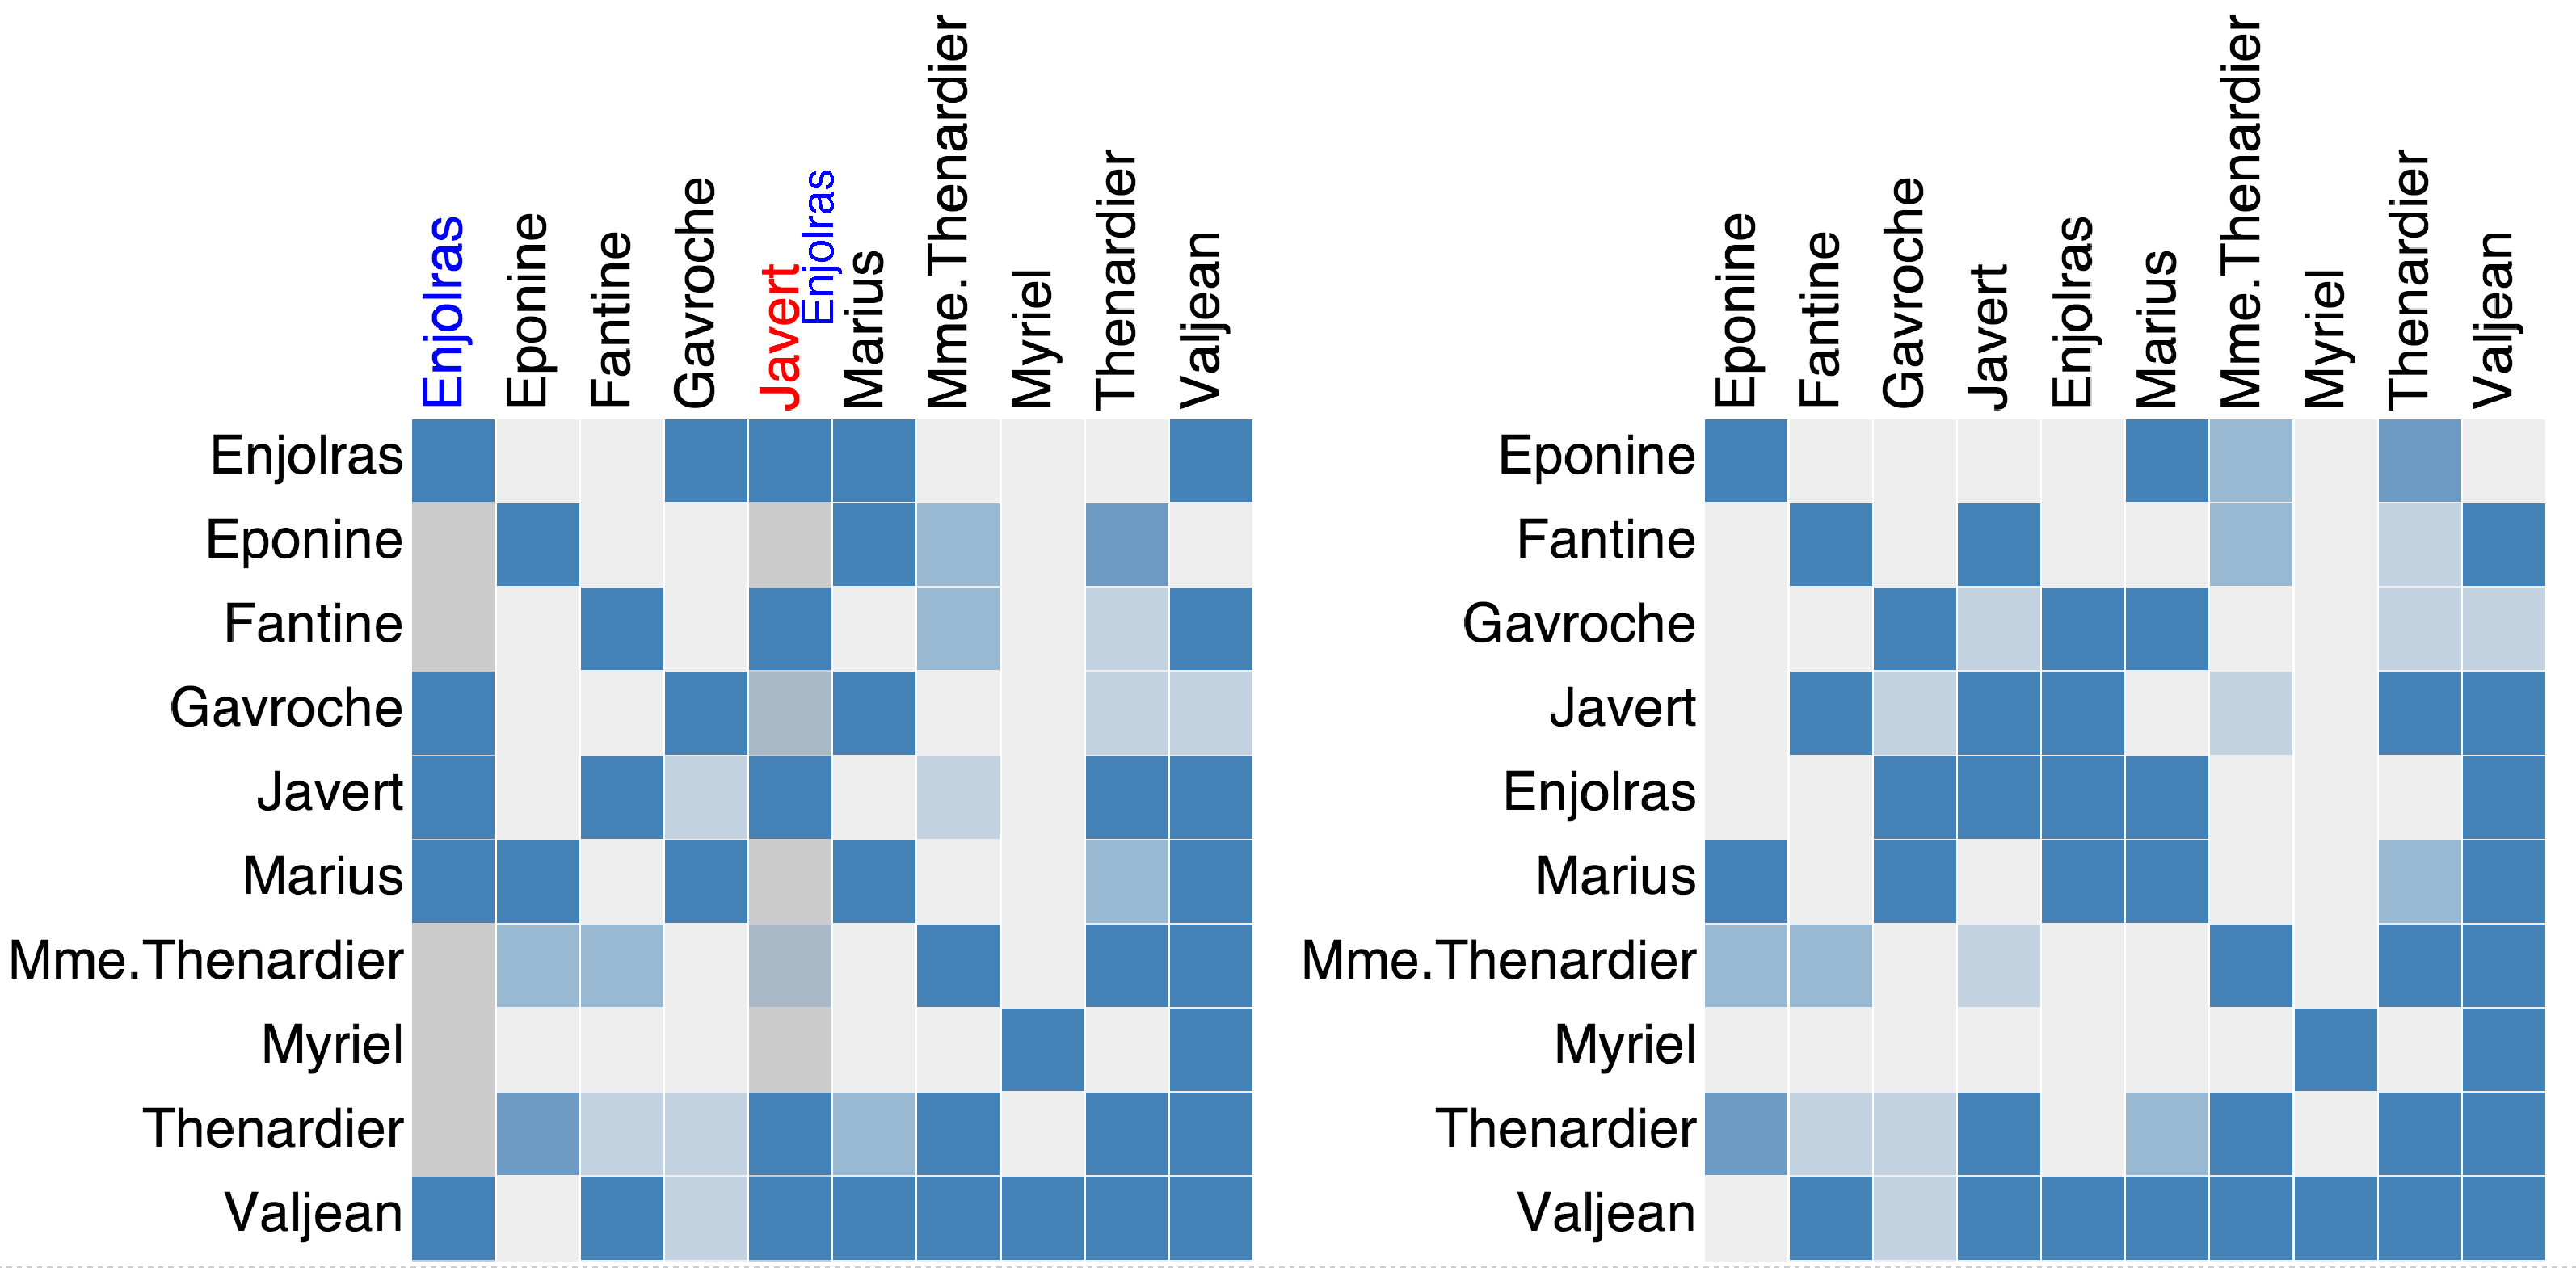
\includegraphics
  [width=0.6\textwidth]{cooccurrence}}
\end{wrapfigure}

\vspace{-7pt}

The figure to the left shows a co-occurrence matrix of Les Mis\'{e}rables
characters. To reorder the columns of the matrix, we first construct a data
source that computes the sort order of characters and initialize it to an
alphabetical ordering. A signal on \texttt{@col\_label:mousedown} captures the
source column to be reordered, while a signal on \texttt{[@col\_label:mousedown,
mouseup] > mousemove} updates the target column location. On \texttt{mouseup},
the data source is updated to swap the two sorting indices.

\vspace{-10pt}

\subsection{Filter: Control Widgets}

\vspace{-7pt}

\begin{figure}[t!]
  \centering
  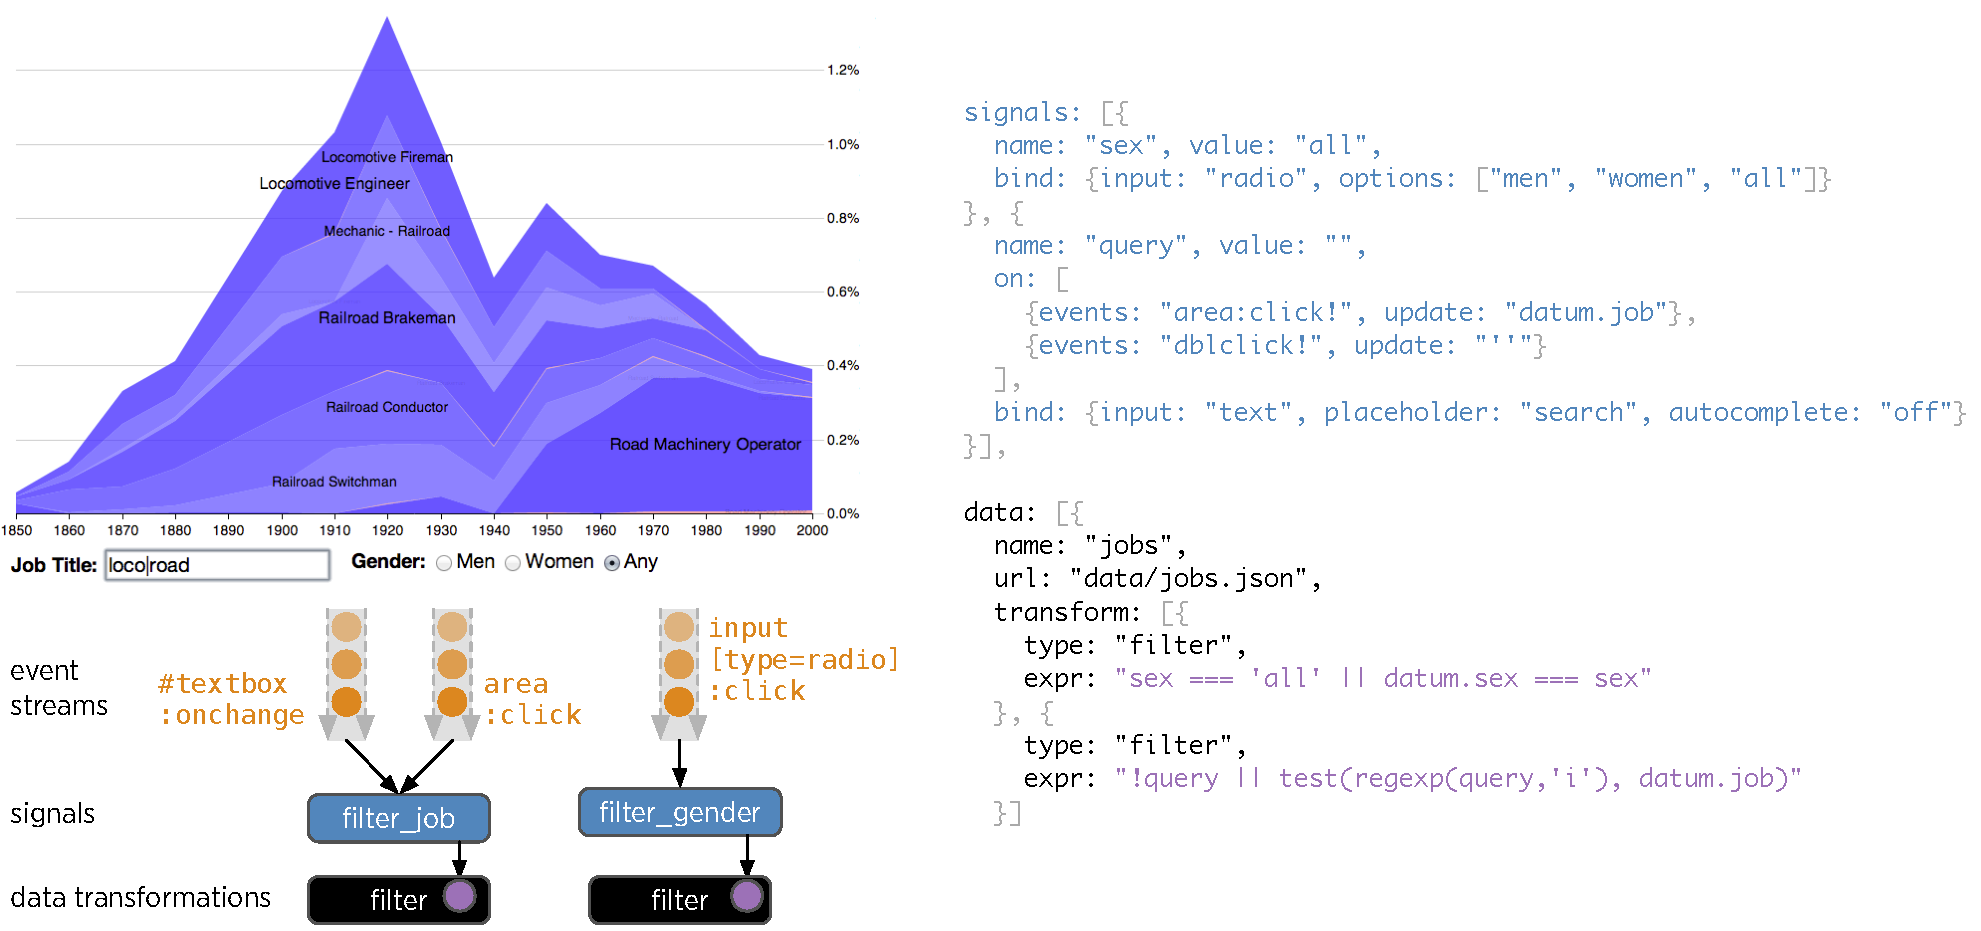
\includegraphics[width=0.9\columnwidth]{jobVoyager}
  \caption{The job voyager can be filtered using signals bound to control
  widgets. The textbox pattern matches against job titles while radio buttons
  filter by gender.}
  \label{fig:vg:jobVoyager}
\end{figure}

\Cref{fig:vg:jobVoyager} shows the Job Voyager~\cite{heer:voyagers}
visualization with control widgets to filter the visualized data. A textbox
allows users to enter search terms to filter job titles, while the radio buttons
allow users to filter by gender. We bind signals to the value of these control
widgets, and then construct predicates attached to filter data transformations.
For the textbox signal, a regular expression tests terms against job titles,
while an equality test filters by gender based on the radio button signal. This
example illustrates how external widgets can easily be bound to our reactive
model.

\vspace{-20pt}

\subsection{DimpVis: Touch Navigation with Time-Series Data}

\vspace{-7pt}

DimpVis~\cite{kondo:dimpvis} is a recently introduced interaction technique that
allows direct manipulation navigation of time-series data. Starting with a
scatterplot depicting data at a particular time slice, users can touch plotted
points to reveal a ``hint path'': a line graph that displays the trajectory of
the selected element over time. Dragging the selected point along this path
triggers temporal navigation, with the rest of the points updating to reflect
the new time. In evaluation studies, users reported feeling more engaged when
exploring their data using DimpVis~\cite{kondo:dimpvis}.

As shown in \cref{fig:vg:dimpvis}, we can recreate this technique with Reactive
Vega's declarative interaction primitives and the GapMinder
country-fertility-life-expectancy dataset used by the original. Input data is
passed through a \texttt{Window} transform, such that every tuple contains
references to the tuples that come before and after it in time, and filtered to
remove triplets that span multiple countries. Signals constructed over mouse and
touch events capture the selected point, and downstream signals calculate
distances between the user's current position and the previous and next points.
A scalar projection over these distances gives us scoring functions that
determine whether the user is moving forwards or backwards in time. Scores feed
a signal that is used in a derived data source to calculate new interpolated
properties for the remaining points in the dataset. These interpolated
properties determine the position of plotted points, producing smooth
transitions as the user drags back-and-forth. To draw the hint map, a derived
data source filters data tuples for the selected country across all years.

\begin{figure}[h!]
  \centering
  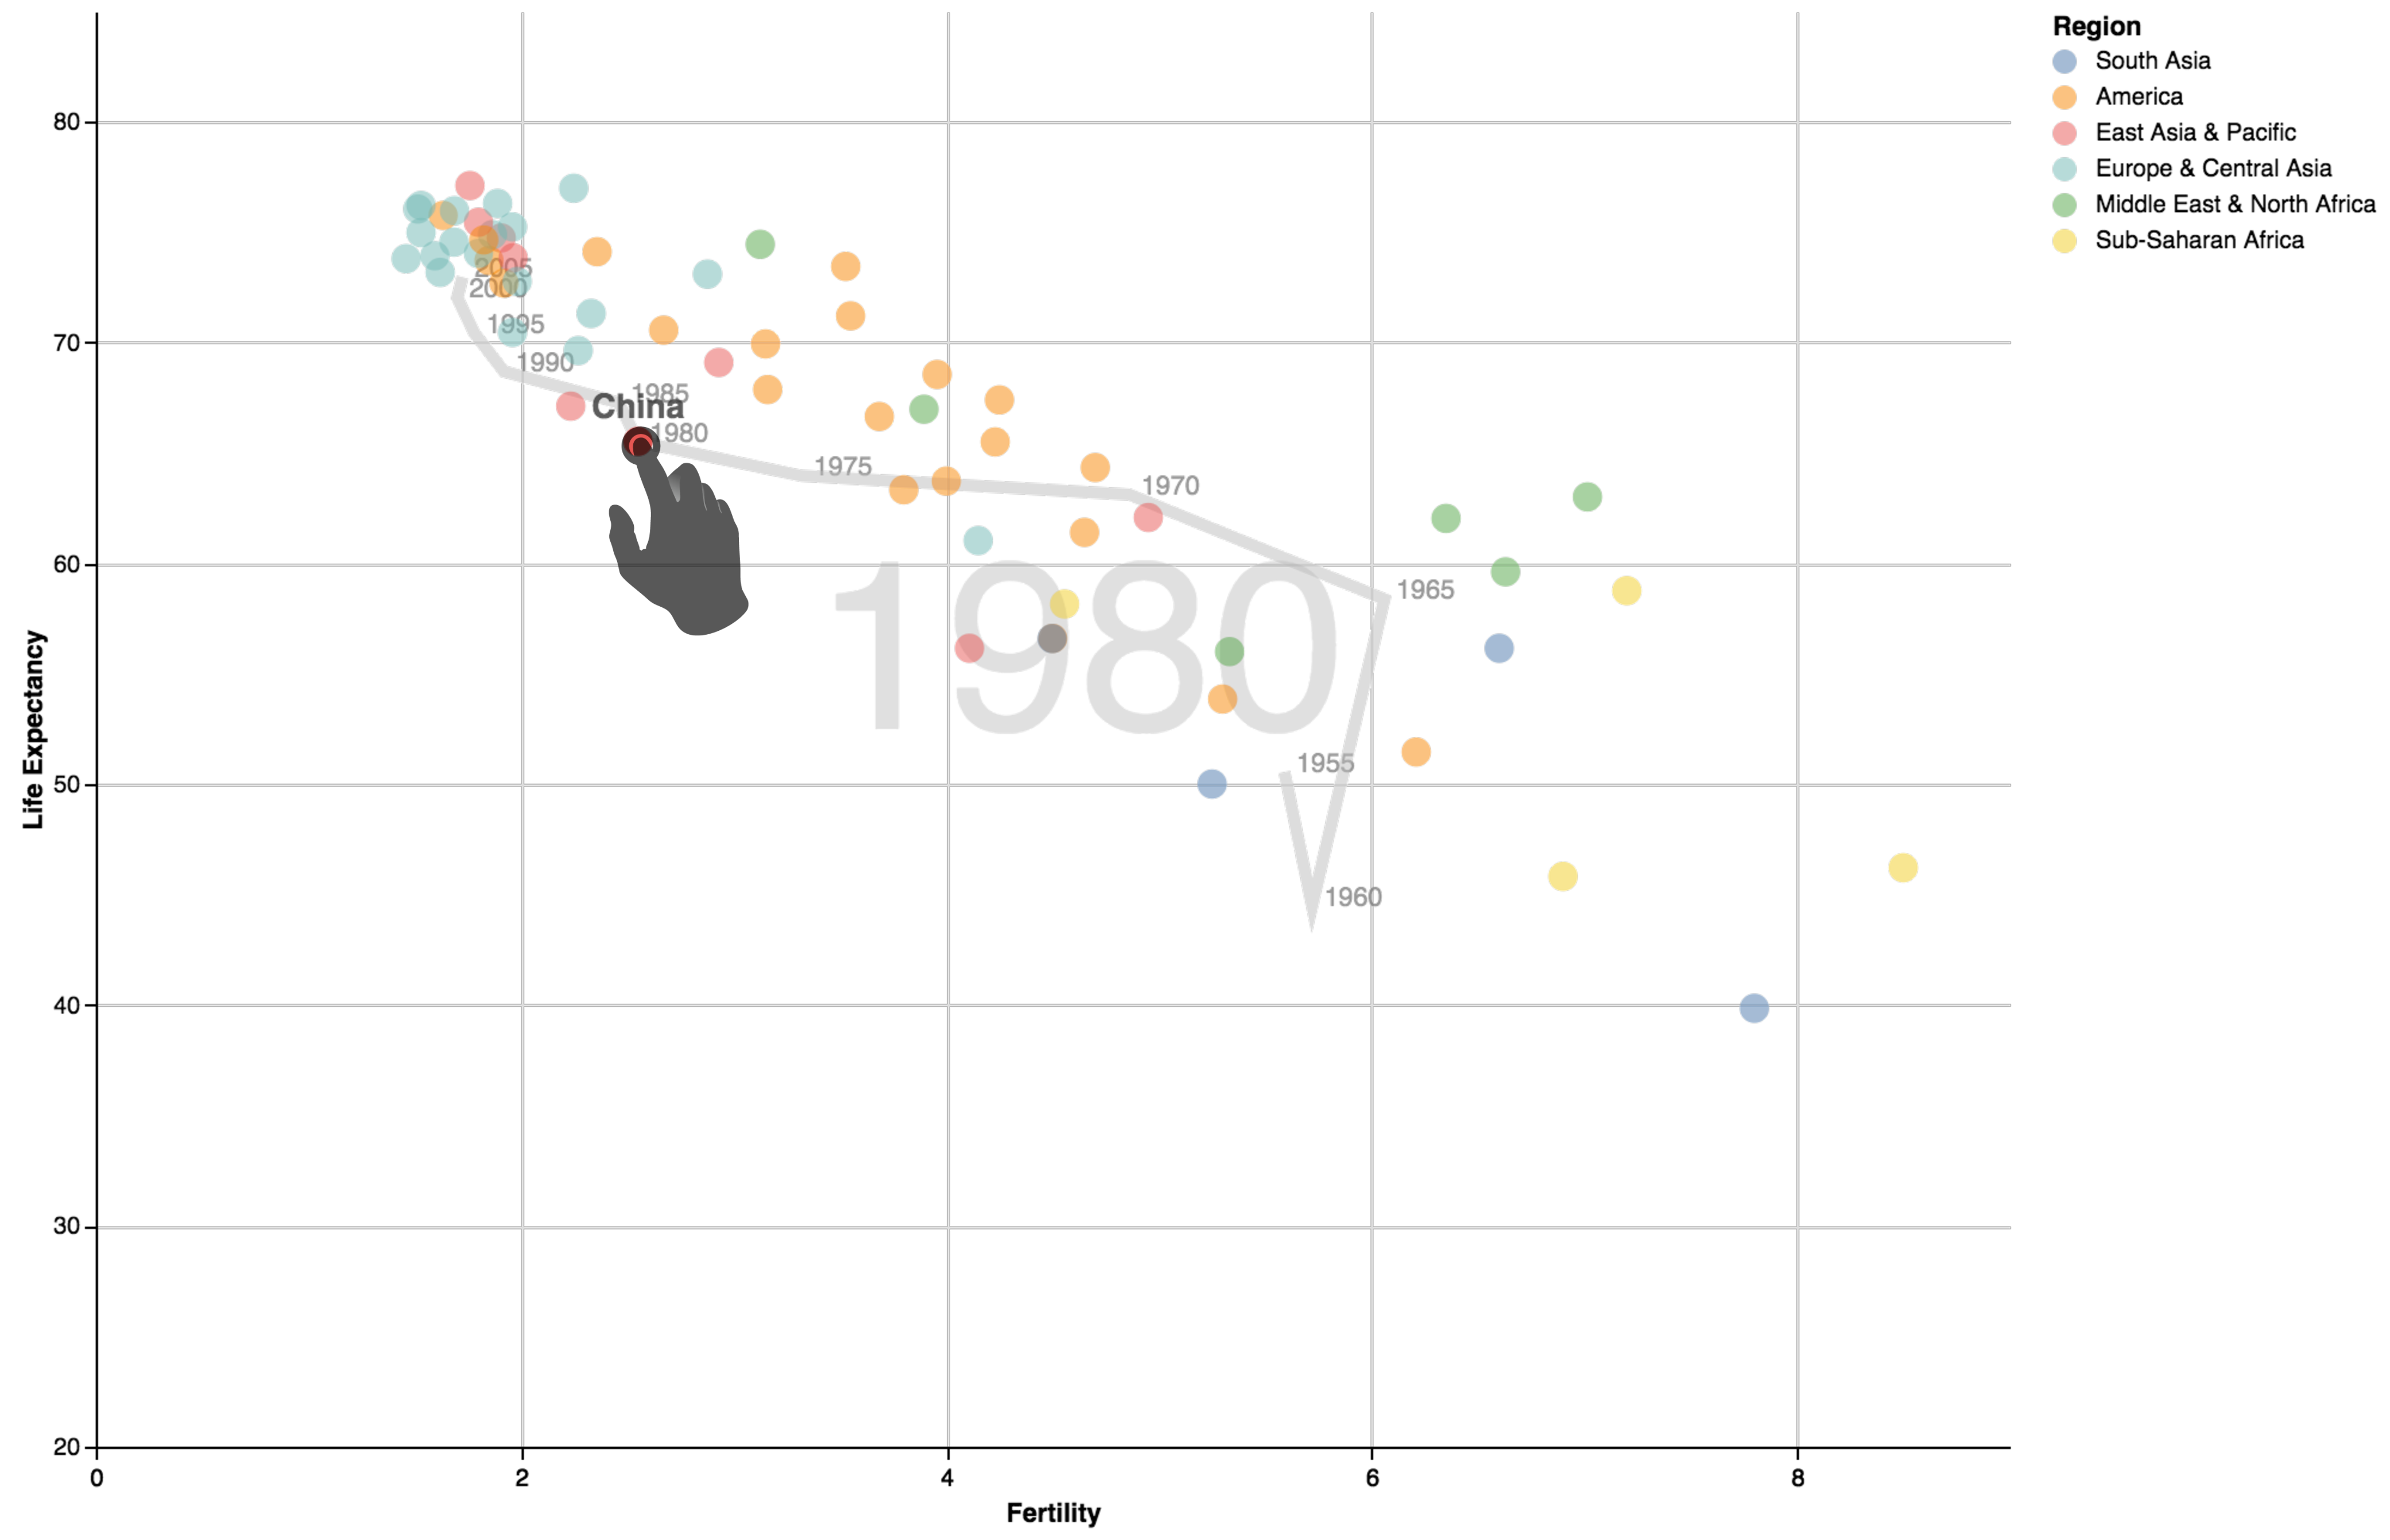
\includegraphics[width=\columnwidth]{dimpvis}
  \caption{DimpVis~\cite{kondo:dimpvis}, touch-based navigation of time-series
  data recreated with Reactive Vega.}
  \label{fig:vg:dimpvis}
\end{figure}

\vspace{-10pt}

\subsection{Reusable Touch Interaction Abstractions}

\vspace{-7pt}

With the proliferation of touch-enabled devices, particularly smartphones and
tablets, supporting touch-based interaction has become an increasingly important
part of interactive visualization design. However, HTML5 only provides a
low-level API for touch events, with three event types broadly
supported\,---\,\texttt{touchstart}, \texttt{touchmove}, and \texttt{touchend}.
On multitouch devices these events contain an array of touch points. The
application developer is responsible for the bookkeeping involved with tracking
multiple points across interactions, a cumbersome and difficult process.

Declarative interaction design enables us to abstract low-level details away,
building reusable interactors that expose higher-level, semantic events as
signals instead. For example, an interactor could define signals that perform
the necessary logic for common multitouch gestures. Once such an interactor is
included in a host visualization, the visualization designer can then safely
ignore lower-level events, and instead build interactions driven by the
interactor's signals\,---\,using \texttt{twotouchmove} and \texttt{pinchDelta}
signals to drive panning and zooming behaviors, for instance.
% !TEX root = ../thesis.tex
\section{Discussion: Cognitive Dimensions of Notation}
\label{sec:vg:discussion}

The previous section demonstrated the expressivity of Reactive Vega's model of
declarative interaction design. Here, we evaluate it from the perspective of a
visualization designer using the Cognitive Dimensions of
Notation~\cite{blackwell:cogdim}, a set of heuristics for evaluating the
efficacy of notational systems such as programming languages and interfaces. Of
the 14 dimensions, we evaluate Reactive Vega against a relevant subset and
compare it against current common practice: declarative specification of visual
encodings using D3~\cite{bostock:d3} and imperative event handling callbacks for
interaction.

\textbf{Abstractions} (types and availability of abstraction mechanisms) and
\textbf{Viscosity} (resistance to change). Streams and signals abstract the
low-level events that trigger interactions and decouple them from downstream
logic. This approach can facilitate rapid iteration: the result of an
interaction can be designed (for example, highlighting points), and then a
variety of different event triggers can be prototyped by simply rebinding the
appropriate signals. As our examples demonstrate, rebinding signals reduces the
burden for resolving conflicting interactions or retargeting to different
platforms. By comparison, iterating with event callbacks can be more difficult.
A particular sequence of events may require a specific ordering of callbacks,
and coordinating the visualization state across these functions falls to the
designer.

\textbf{Premature Commitment} (constraints on the order of doing things).
Abstracting streams into signals does impose a premature commitment. Users must
define them before they are able to use any lower-level events to trigger state
changes. This requirement could be relaxed: users could use event streams
inline, for example within a predicate or production rule. However, we believe
such inline references are a poor design pattern as they make an interaction
technique dependent on a specific set of events\,---\,a common problem with
existing interactor typologies. Moreover, reuse would be hampered as it would
become more difficult to resolve conflicting interactions (e.g., brushing and
panning) or retarget techniques across input modalities.

\textbf{Hidden Dependencies} (important links between entities are not visible).
Signals do introduce hidden dependencies as they obscure which input events
trigger particular changes to the state of the visualization. However, we
believe that the gains in viscosity outweigh the complexities of these hidden
dependencies, particularly as the latter can be ameliorated by naming signals
appropriately. Furthermore, as our code examples illustrate, all the factors
that directly affect a particular state are captured within a single Reactive
Vega specification. For example, a signal definition specifies all events or
signals that may affect its value; similarly, a visual property may use a rule
which enumerates all the values it may take. With D3, the visual encoding
specification may not completely define all states. Instead, the user must trace
a flow through event callbacks, a process further exacerbated by an
unpredictable execution order. The user is forced to coordinate interleaved
callbacks, introducing \textbf{hard mental operations} and
\textbf{error-proneness}.

\textbf{Consistency} (similar semantics are expressed in similar syntactic
forms). Our interaction model is best suited for systems that declaratively
specify visual encodings, and would feel foreign in imperative systems. However,
given the widespread adoption of D3, and Vega's increasing integration in
systems~\cite{lyra, voyager, wikipedia:graph} we believe this is not a
significant liability. By contrast, registering event callbacks on D3
visualizations breaks consistency: visual design is declarative while
interaction design is imperative. It requires users to think in terms of
different notational systems, and exposes underlying implementation and
execution concerns.

\textbf{Visibility} (ability to view components easily). One of the primary
advantages of using D3, and registering event callbacks, is being able to debug
code directly within a web browser~\cite{bostock:d3}: the generated
visualization can be inspected, while the JavaScript console can be used to
interactively debug event callbacks. Reusing such existing scaffolding is more
difficult with Reactive Vega as its runtime, which parses and renders a
specification, introduces its own stack of abstractions. However, we believe
this gap offers a promising avenue for future work in new development
environments that can leverage Vega's reactive semantics. For instance, initial
work by Hoffswell et al.~\cite{hoffswell:debugging} has devised a
``time-travelling'' debugger for Reactive Vega specifications. In particular,
the authors note that signals are a critical abstraction barrier, providing a
meaningful entry-point into an interaction specification. To construct a similar
debugger for imperative event handling callbacks would require complex static
analysis to identify and surface relevant program state.

In summary, Reactive Vega introduces hidden dependencies between state changes
and their triggering input events and, without additional tooling, decreases
visibility into runtime execution. However, we believe these drawbacks are
outweighed by the increase in specification consistency between visual encodings
and interaction, and a decrease in viscosity, allowing users to iterate more
quickly over interaction design.

\section{Summary}
\label{sec:vg:lang-summary}

In this chapter, we demonstrate that the advantages of declarative specification
extend to interaction design as well. With event streams and signals, users need
only describe the relationship between input events and interactive state
respectively. Reactive semantics ensure that this state no longer needs to be
manually maintained by users, but is automatically updated when new events
occur. Moreover, signals provide a powerful abstraction barrier that simplifies
retargeting and has spurred development of a new ``time-traveling''
debugger~\cite{hoffswell:debugging}. Reusing and repurposing interactive
behaviors is also supported by passing predicates through scale inversions, and
extracting declarative specifications to standalone interactors.
